\let\TeXyear\year
\documentclass{ieeeaccess}
\let\setyear\year
\let\year\TeXyear

\usepackage{cite}
\usepackage{amsmath,amssymb,amsfonts}
\usepackage{algorithm,algorithmic}
\usepackage{graphicx}
\usepackage{textcomp}
\usepackage{caption}
\usepackage{helvet}  
\usepackage{comment}
\usepackage{pgfplots}
\usepackage{pgfplotstable}
\usepackage{listings}
\usepackage{booktabs}
\usepackage{siunitx}
\usepackage{setspace}
\usepackage{array}

\newcolumntype{L}[1]{>{\raggedright\let\newline\\\arraybackslash\hspace{0pt}}m{#1}}
\newcolumntype{C}[1]{>{\centering\let\newline\\\arraybackslash\hspace{0pt}}m{#1}}
\newcolumntype{R}[1]{>{\raggedleft\let\newline\\\arraybackslash\hspace{0pt}}m{#1}}

\pgfplotsset{compat=1.7}
\setyear{2023}
\NewSpotColorSpace{PANTONE}
\AddSpotColor{PANTONE} {PANTONE3015C} {PANTONE\SpotSpace 3015\SpotSpace C} {1 0.3 0 0.2}
\SetPageColorSpace{PANTONE}

\newtheorem{Problem}{Problem}
\newtheorem{Definition}{Definition}

\def\BibTeX{{\rm B\kern-.05em{\sc i\kern-.025em b}\kern-.08em
    T\kern-.1667em\lower.7ex\hbox{E}\kern-.125emX}}

\captionsetup{font={sf,small,stretch=0.80},labelfont={bf,color=accessblue}}

\begin{document}
\history{Date of publication xxxx 00, 0000, date of current version xxxx 00, 0000.}
\doi{10.1109/ACCESS.2017.DOI}

\title{Visualize Knowledge Graphs through semantic maps}
\author{\uppercase{P. Camarillo-Ramirez}\authorrefmark{1},
\uppercase{L. F. Guti\'{e}rrez-Preciado\authorrefmark{1}, and F. Cervantes-Alvarez}.\authorrefmark{1}}
\address[1]{Western Institute of Technology and Higher Education, Tlaquepaque, Jalisco 45601 Mexico (pablo.camarillo@iteso.mx;lgutierrez@iteso.mx;fcervantes@iteso.mx)}

\tfootnote{This work was supported in part by the  National Council of 
Science and Technology of Mexico through grant 498322}

\markboth
{Author \headeretal: Preparation of Papers for IEEE TRANSACTIONS and JOURNALS}
{Author \headeretal: Preparation of Papers for IEEE TRANSACTIONS and JOURNALS}

\corresp{Corresponding author: P. Camarillo-Ramirez (e-mail: pablo.camarillo@iteso.mx)}

\graphicspath{ {img/} }

\begin{abstract}
Knowledge Graphs (KGs) are one of the most novel technologies used to
improve search engines and support
decision making in the life sciences since they structure information in graph form
by encoding concepts as nodes, and the semantics of the relationship
among concepts as edges. The analysis of KGs calls
for an effective strategy to visualize them. However, the increasing
size of KGs makes the exploring process a big challenge.
A semantic map is a visual representation of related concepts that helps humans
in the learning process. In this work, we propose to generate a simplified visual
representation of a KGs by generating semantic maps. We apply several clustering 
algorithms to group the \textit{related} concepts in KGs. We used different semantic similarity
metrics to compute the matrix consumed by the clustering algorithms.

\end{abstract}

\begin{keywords}
Knowledge graphs; Knowledge graphs visualization; Semantic similarity; Semantic mapping; Big Data;
\end{keywords}

\titlepgskip=-15pt

\maketitle

\section{Introduction}
\label{sec:introduction}

Knowledge Graphs are considered one of the emerging technologies associated
with Big Data by providing semantic structured information that can be 
interpreted by machines, and such attribute is used to speed up the production
of more intelligent systems \cite{Zou_2020}. The core idea behind a Knowledge 
Graph (KG) is to represent knowledge from real world in a graph structure, 
where nodes represent entities of interest and edges represent relations 
between these entities \cite{Hogan21}. Recently, 
academic and private organizations have constructed KGs, such as YAGO 
\cite{suchanek2007yago}, DBPedia \cite{auer2007dbpedia}, Freebase 
\cite{Freebase08}, NELL\cite{NELL10}, Google Knowledge Graph 
\cite{GoogleKG12}, Microsoft Satori \cite{Satori13}, Facebook Entity
Graph \cite{Facebook13}, and Wikidata \cite{Wikidata14}, which contain
millions of entities and billions of relationships. The main applications 
of KGs include the enhancement of search engines like Google \cite{GoogleKG12}
or Bing \cite{Satori13}, question answering \cite{Chen2022}, information 
retrieval, recommender systems \cite{Lin2022, Haotian2022}, domain-specific KG 
building \cite{Zhang2022, Borrego2022, Guan2022}, and decision support in the 
life sciences \cite{Zou_2020,Belleau08,Ruttenberg09,Momtchev09}.

Considering the continuous increase in the use of KGs in 
decision-making applications, it becomes important to 
provide explanations for the results generated by the 
graph. Visualizing KGs can help to unlock insights from 
data and facilitate better decision making, actually 
visual data exploration is considered as a 
hypothesis-generator process by allowing users to gain
a deep understanding of the data \cite{keim2001visual},
hence producing an effective visual representation of 
a KG is crucial to understand relationships between 
entities and concepts in a domain. By representing the
information in a visual format, users can quickly identify
patterns, trends, and clusters or related information 
that may be difficult to see in a text-based representation. 
Existing approaches to visualize KGs are focussed on 
drawing the whole structure \cite{gomez2018visualizing} 
preventing data analysts to explore the KG beyond its 
structural information.

Semantic maps, on the other hand, are a technique widely
used to understand complex topics and consists of a 
categorical structuring of information in a graphic form 
\cite{johnson1986semantic}. Semantic maps have a central
word indicating the main topic of the map and it is
connected with a set of keywords that groups the rest
of the vocabulary.In this paper, we hypothesize that 
semantics maps are useful to visualize the high level 
of abstraction of a KG based on the semantic closeness of 
entities in the KG. To generate a semantic map it is 
necessary to find the groups of related instances. Unsupervised
learning provides clustering algorithms to classify
data into one or more classes depending on a similarity
or distance  measure \cite{SCHAEFFER200727}. Theoretically, 
if a clustering strategy is applied over the set of 
entity instances of a KG, it will group those entity
resulting groups can be used to build the semantic 
map. Section \ref{sec:results} presents a set of 
experiments validating the above notion.

The main contribution of this work is to provide a 
formal definition of the semantic map of a KG as well
as a strategy to measure the quality of these semantic 
maps by running a set of experiments showing that 
these semantic maps can be useful to provide a high-level
view of a KG.

The rest of this paper is structured as follows. 
Section \ref{sec:KG}, we introduce KGS. In Section
\ref{sec:related}, we review the most relevant literature
associated with knowledge graph visualization, graph
clustering, semantic similarly, and semantic mapping
topics. Section \ref{sec:Method}, describes the proposed
method and algorithms needed to generate the semantic
maps of a KG. Section \ref{sec:results} discusses the
results obtained from a set of experiments evaluating 
the process of generating semantic maps generated 
from a collection of datasets extracted from 
DBPedia. Finally, Section \ref{sec:conclusions} presents
final remarks and future work.

\section{Foundations of Knowledge Graphs}
\label{sec:KG}

Some definitions describe a KG as a graph-structured
knowledge base \cite{nickel2015review, 
seufert2016instant}. In this work, we consider a knowledge
base a set of sentences/facts expressed in some 
formal language such as description logic. In other words, 
KGs consist in a collection of facts formed by $<subject,
predicate,object>$. These collections are typically 
represented in languages, such as RDF (Resource Description
Framework) \cite{RDF}, OWL (Ontology Web Language) \cite{OWL},
or N-Triples which is a subset of the more complex RDF/XML syntax,
and is designed to be human-readable as well as 
machine-readable. It is a plain text format that represents 
RDF statements using subject-predicate-object triples, with
each element separated by whitespace and terminated by a 
period.

According to description logic terminology, knowledge bases 
have two types of axioms: a terminology box (TBox) and an 
assertion box (ABox) \cite{horrocks2008ontologies}, hence a 
KG should contain these two sets of axioms to be considered
as a knowledge base. To exemplify the above idea, Figure 
\ref{Fig:TboxAndAbox} shows sets TBox and ABox of a group 
of entities and relationships extracted from DBPedia
\cite{auer2007dbpedia} \footnote{https://dbpedia.org}. In 
KGs, the ontology classes (e.g.,\texttt{dbo:Book} 
\footnote{URIs mentioned in this document use the common 
prefixes described in https://prefix.cc} or \texttt{dbo:Movie})
correspond with the TBox and describe concepts hierarchies, 
while the ontology instances correspond with the ABox 
and describe entity instances (e.g.,\texttt{dbr:Lucasfilm} or \texttt{dbr:George\_RR\_Martin}) and their
relationships.  Hierarchical relationships like \textit{is a}
defines the connection between each pair of concepts in TBox. 
For example, axioms (\texttt{dbo:Book}, \textit{is a}, 
\texttt{dbo:Work}) and (\texttt{dbo:film}, \textit{is a}, 
\texttt{dbo:Work}) describe the fact that both \texttt{dbo:Book} 
and \texttt{dbo:film} concepts are descendants of the class
\texttt{dbo:Work}. Alternatively, in ABox, axioms also
indicate the list of types that one entity instance may
have. For instance, in Figure \ref{Fig:TboxAndAbox}, the axiom (\texttt{dbr:A\_dance\_of\_dragons}, \textit{rdf:type},
\texttt{dbo:Book}) indicates that resource
\texttt{dbr:A\_dance\_of\_dragons} is an instance of class
\texttt{dbo:Book}. Another type of axioms in ABox like
(\texttt{dbr:George\_RR\_Martin}, is \textit{dbo:creator\_of}
of, \texttt{dbr:DaenerysTargaryen}) and 
(\texttt{dbr:George\_RR\_Martin}, is \textit{dbo:author} of,
\texttt{dbr:A\_dance\_of\_dragons}) indicate
that the instance \texttt{dbr:George\_RR\_Martin} has two semantic
connections with \texttt{dbr:DaenerysTargaryen} and 
\texttt{dbr:A\_dance\_of\_dragons} entity instances.

\Figure[h!](topskip=0pt, botskip=0pt, midskip=0pt)[width=0.95\textwidth]{img/TBoxAndAbox.pdf}
{Small group of concepts and instances extracted from DBPedia. \label{Fig:TboxAndAbox}}

Let us propose a formal definition of KG before describing
the rest of relevant topics associated with the semantic 
mapping process described in this paper.

\begin{Definition}[Knowledge Graph]
Given a set of entities $V$, a set of property labels $L$,
and a set of edges $E$ a Knowledge Graph $K$ is defined as
$K = (V, L, E)$ where $E$ is a subset of the cross
product of entities and property labels defined as 
$V \times L \times V$. Each member of $E$ is referred to as a
triple $(subject-property-value)$.
\end{Definition}

\section{Related work}
\label{sec:related}

This section describes the most relevant concepts associated to
the proposed semantic mapping process.

\subsection{Visual Data Exploration of knowledge graphs}
The idea behind the visual data exploration process is to present 
the data in some visual form, allowing users to draw conclusions 
of the analyzed phenomena \cite{keim2001visual}. This process, also
known as the \textit{information seeking mantra}, follows three steps: overview,
zoom and filter, and details-on-demand \cite{Shneiderman96}. In this
context, ontologies are considered one of the most relevant data
visualization techniques. In the field of computer science, an ontology
is a model for describing the world that consists of a set of types,
properties, and relationship types \cite{Garshol2004MetadataTT}
and by providing an initial attempt to visualize linked data.

In regard to visual exploration of KGs, challenges include context
adaptation, users input \cite{Koutra2019}, data heterogeneity
\cite{OntoVis,6787141,1703364}, supporting diverse analysis tasks 
(query, combination, filtering, etc.), and performance
\cite{gomez2018visualizing}. In this study, semantic mapping proposal
is to combine and reduce the number of edges in the KG using the 
semantic similarity among its entities to compute clusters of related
entities.


Recent applications have proven useful for large graph visualizations 
to understand different phenomena, such as Bitcoin transactions 
\cite{mcginn2016visualizing} and online discussions
\cite{molina2017improving}. For big knowledge graphs, it is necessary a
distributed implementation of the layout algorithms to improve the time 
needed to generate the visual representation
\cite{gomez2018visualizing}. Actually, Consalvi et. al \cite{Consalvi2022} 
propose a self-contained system to compute interactive visualizations of
thousands elements in a mobile browser.

In addition of recent efforts on KGs visualization, there are some commercial
products enabling analysts to visualize RDF graphs like Data
Graphs\footnote{https://datagraphs.com} or the 
family of tools developed by Cambridge Intelligence company: Keylines, 
ReGraph, and KronoGraph \footnote{https://cambridge-intelligence.com/}
that offer the capability to render KGs to support tasks in areas like 
pharmacy and bio-science research or financial analysis. In the area of 
free tools, there are two online tools that consumes RDF data and produce 
a visual representation: RDF visualizer
\footnote{https://issemantic.net/rdf-visualizer}
and RDF grapher \footnote{https://www.ldf.fi/service/rdf-grapher}. The
main limitation with these tools is the small amount of data they
can process.

\subsection{Knowledge Graph summarization}

Recent works \cite{6787141,1703364,8801911}
have shown that visualizing a simplified version of a large graph is an
adequate alternative. In the context of data mining, summarization is the
process of facilitating the identification of meaningful data. The
applications of graph summarization include reduction of data
volume and storage, speedup of graph algorithms and queries, interactive
analysis support, and noise elimination \cite{liu2018graph}. Recently, it
has been proposed to summarize large graphs in order 
to enable an efficient visualization of their content. For example, in 
\cite{Koutra2019}, the authors focus on summarizing KGs by taking
advantage of individual interests to generate personalized knowledge graph
summaries. In \cite{OntoVis}, Shen et al. propose a visual 
analytics tool called OntoVis, which performs both structural and semantic
abstractions to offer a summarized version of a large graph and thus
being able to visualize a simplified version of the graph. Another
related work is presented in \cite{koutra2014vog}, which describes the VoG
(Vocabulary-based summarization of Graphs) algorithm to summarize and
understand large graphs by constructing and visualizing subgraph-types, 
such as starts, cliques, and chains. The visual abstraction presented in
\cite{8801911}, transforms geo-tagged social media data into high-dimensional
vectors by utilizing a doc2vec model.

Regardless of the application, one of the main challenges of
graph summarization is defining which data is of interest. Every
summarization strategy depends on selecting an interest criteria to
extract meaningful information \cite{liu2018graph}. However, to achieve a 
concise definition of \textit{interesting} is not an easy task. For
example, the FUSE algorithm \cite {Seah12} proposes a profit maximization
model that seeks to find a summary by maximizing information profit under
a budget constraint. On the other hand, VoG \cite{koutra2014vog} exploits
the Minimum Description Length (MDL) principle aimed at identifying the
best subgraphs by choosing those which save most bits. In the case of
semantic abstraction proposed in \cite{8801911}, a dual-objective blue 
noise sampling model is utilized to select a subset of social media data
items supporting the spatial distribution and semantic correlation for
the resulting simplified geographical visualization. The personalized 
summaries of KGs described in \cite{Koutra2019}, the criteria to decide 
which information is \textit{interesting} for each user is determined by
reviewing the users' query history. The work of M. Tasnmin et al. 
propose a strategy to find equivalent entities in a KG using the context 
of each RDF Molecule \cite{Tasnim2020}. Semantic mapping process described
in this document uses the semantic similarity between each pair of entity
instances in the KG to infer the groups of related instances.

\subsection{Semantic maps}

A semantic map is a type of graphical representation that shows the 
relationships between different concepts or words within a particular 
domain or field of study. The purpose of a semantic map is to visually 
organize and display the meaning and connections between various terms 
or concepts, highlighting their semantic similarities and differences. 
In other words, a semantic map provides a visual representation of how 
different ideas or concepts are related to each other and how they are
grouped together based on their shared meanings or semantic properties. 
Figure  \ref{fig:example_semantic_map} shows an
example of a semantic map describing the topic \textit{Water}. It
contains three node categories: (1) the central words (root), (2)
the set of keywords (e.g., Usages, Living things, etc.), and (3) the
vocabulary associated to each keyword, for instance, words
\texttt{Cooking} and \texttt{Bathing} are associated with keyword 
\textit{Usages}.

\Figure[h]()[scale=0.35]{img/Water_Semantic_Map_no_colour.pdf}
{Example of a semantic map of concepts and vocabulary  associated with
topics \textit{Water}.\label{fig:example_semantic_map}}

\subsection{Semantic similarity}

The semantic similarity is a metric used in Natural Processing Language 
(NPL) and Information Retrieval (IR) areas \cite{HOVY20132} that
represents how related are two concepts based on their hierarchical 
relations \cite{resnik1995using}, \cite{turney2010frequency}. 
In a KG, the semantic similarity between two entities $e_{1}, e_{2} \in V$
is denoted as $sim(e_{1}, e_{2})$. Intuitively, semantic distance between
two words is the most easy way to calculate semantic similarity and it is
usually determined by the path connecting two entities in KG. Existing 
semantic similarities metrics are classified in two main groups: corpus-based 
and knowledge-based approaches \cite{mihalcea2006corpus}. Corpus-based 
similarity metrics are focused on learning how similar are two concepts based 
on the information from large corpora. Two examples of corpus-based similarity
metrics are pointwise mutual information \cite{church1990word}, and latent 
semantic analysis \cite{landauer1997solution}. In contrast, knowledge-based
similarity metrics quantify the degree to which two words are 
semantically related \cite{budanitsky2001semantic}. In KG, knowledge-based
approaches, semantic similarity is determined using the information provided 
by the TBox. Knowledge-based approaches include path-based metrics such as
those proposed by Hulpus et at. \cite{hulpucs2015path}, Wu $\And$ Palmer
\cite{wu1994verb}, and Leacock $\And$ Chodorow \cite{leacock1998combining}.
Other knowledge-based measures utilize the Information Content (IC) metric like 
Lin \cite{lin1998information}, Jiang and Conrath \cite{jiang1997semantic}, 
and Resnik \cite{resnik1995using} metrics. IC of concepts is a statistical
measure that computes the specificity of a concept over a corpus. Higher 
values of IC indicate more specific concepts (e.g., \texttt{dbo:Book}) and lower 
values of IC are associated with more general concepts (e.g., \texttt{owl:Thing}).
Hybrid knowledge-based approaches like IC-graph \cite{ZhuIglesias2017} or Zhou
\cite{zhou2008new} combine IC and some other metrics to compute how related two 
words are. For instance, graph-based IC \cite{ZhuIglesias2017} uses 
the counting services provided by DBPedia and it is calculated using the 
following expression:

\begin{equation}
    IC_{graph}(c_{i}) = -logProb(c_{i})
\end{equation}

Where $Prob(c_{i}) = \frac{freq_{graph}(c_{i})}{N}$ and $N$ is the 
number of entities in the KG. Let $\mathcal{E}(c_{i})$ the set of 
entities having type of $c_{i}$, the frequency of concept $c_{i}$
in the $KG$ is defined as $freq_{graph}(c_{i}) = |\mathcal{E}(c_{i})|$.

\subsection{Centroid-based Clustering}

There exist several techniques to clustering data and recent surveys
summarize these clustering approaches based on the application or
the type of data to group \cite{Dongkuan2015}, 
\cite{DBLP:books/crc/aggarwal2013}, \cite{firdaus2015survey}. Types of
clustering include Centroid-based, Density-based, Distribution-based, and
Hierarchical clustering \cite{google_2022}.

One of the phases of the semantic mapping process is to collocate each entity
into the most appropiate cluster based on its semantic similarity. Each 
resulting cluster needs a node that represents all entities contained on it. We
denote the set of this representing nodes as the keywords of the semantic map. 
Considering these keywords as centroids of clusters, the usage of a centroid-based
clustering is crucial.

The main idea of centroid-based clustering is to find \textit{k}
centroids (or centers) followed by computing \textit{k} sets of data
points that minimize the proximity with each center. For instance, 
K-means algorithm tries to minimize the sim of the squared distance 
between the data points and the cluster's centroid \cite{macqueen1967classification}. 
A variation of K-means is the PAM (Partitioning Around Medoids) algorithm 
that minimizes dissimilarities between points in a cluster and the centroids 
\cite{kaufmanPAM}. The CLARA (Clustering Large Applications) algorithm is 
an extension of PAM for large datasets \cite{kaufmanCLARA}. On the 
other hand, CLARANS (Clustering Large Applications based on RANdomized 
Search) is a partitioning algorithm focused on spatial data mining 
because it recognizes patters and relationships existing in spatial 
data such as topological data \cite{ng2002clarans}. One last 
centroid-based clustering algorithm is the Affinity Propagation (AP) 
algorithm which consists on a message-passing procedure that looks 
for broadcasting messages of attractiveness and availability among 
data points \cite{frey2007clustering}.

\subsection{Cluster quality}

Literature offers two classes of clustering validation
measures: external  clustering validation and internal
clustering validation \cite{DBLP:books/crc/aggarwal2013}. 
Internal validation metrics evaluate the quality of a 
clustering algorithm based on its intrinsic 
properties, while external validation methods evaluate
the quality of a clustering solution based on its agreement
with a known label of the data. Since there is no known
label of the datasets used in the experiments described
in this work, our proposal is to use internal validation
measures such as Silhouette score, Davies-Bouldin score, 
and Calinski-Harabasz Index.

Each internal validation metric measure different aspects
of the clusters. For example, Silhouette score measures
how well each data point fits into its assigned cluster 
compared to other clusters \cite{kaufmanPAM}. Inertia of 
a cluster, also known as the within-cluster sum of squares
(WSS) metric measures how tightly packed the data points
are within each cluster. The goal is to minimize inertia, 
which is equivalent to maximizing the distances between
clusters. On the other hand, Dunn index measures the distance between the nearest points in different clusters and the
distance between the farthest points in each cluster 
\cite{dunn1974well}. Another known quality measure is 
the Davies-Bouldin index which measures the similarity 
between each cluster and its closest neighboring cluster,
while also considering the cluster's internal similarity 
\cite{davies1979cluster}. Finally, Calinski-Harabasz 
index measures the ratio of between-cluster variance 
to within-cluster variance \cite{calinski1974dendrite}.

\section{Proposed method}
\label{sec:Method}

\Figure[h!](topskip=0pt, botskip=0pt, midskip=0pt)[width=1\textwidth]{img/origin.pdf}
{Visual representation from a small KG containing some fictional characters by George R.R. Martin. a) Contains the visual representation produced by Gephi. b) Inferred semantic map of the original KG.\label{Fig:DefaultVisualization}}

The notion behind the semantic map of a KG is to produce 
a reduced version of the KG by exploiting the semantic 
similarity between each pair of entities. To illustrate 
this idea, let us generate a small KG from DBPedia containing 
the list of some fictional characters from series of fantasy novels 
by the novelist George R. R. Martin. Figure \ref{Fig:DefaultVisualization}a) 
presents a visual representation produced by Gephi\footnote{https://gephi.org/}, 
which is one of the most used tools to visualize networked data. However, 
this kind of visualization is not visually super informative 
or visually appealing which may lead in an ineffective
exploratory visual analysis. On the contrary Figure \ref{Fig:DefaultVisualization}b)
shows a semantic map of the KG by grouping the entity instances
and showing the central concept of the map that connects the centroids of
the cluster.



\subsection{Clustering entities of Knowledge Graphs}

The first phase of the semantic mapping process is to
group the entities of the KG based on the semantic 
closeness between each pair of entities in the KG. 
The main challenge of this phase is to extract 
numeric data from the KG and generate a set of
groups of entities. Algorithm \ref{alg:matrix}
describes the process to compute the distance
semantic matrix $D$. 

\begin{Definition}[Semantic distance matrix]
Given a Knowledge Graph $K = (V, L, E)$, and $sim(e_{1}, 
e_{2})$ the semantic similarity between entities $e_{1}$ 
and $e_{2}$, the semantic similarity matrix $D(K)$ represents 
the semantic distance between each pair of entities in $K$ i.e., 
the value for cell  $d_{i,j} = 1 - sim(e_{i}, e_{j})$.
\end{Definition}

\begin{algorithm}
 \caption{Algorithm to build the semantic distance matrix}
 \label{alg:matrix}
 \begin{algorithmic}[1]
 \renewcommand{\algorithmicrequire}{\textbf{Input:}}
 \renewcommand{\algorithmicensure}{\textbf{Output:}}
 \REQUIRE List of triples $T = {t_{1}, \dots, t_{n}}$
 \ENSURE  Semantic distance matrix $D$
  \FOR {$i = 1$ to $n$}
  \FOR {$j = i$ to $n$}
  \IF{$i = j$}
  \STATE $D(i, j) = 0$
  \ELSE
  \STATE $D(i,j) = D(j, i) = sim(t_{i}, ts_{j})$
  \ENDIF
  \ENDFOR
  \ENDFOR
 \RETURN $D$ 
 \end{algorithmic} 
 \end{algorithm}

The relation between similarity and distance follows 
the notion that the higher is the similarity between 
two entities the lower is the distance between these 
entities. The $i-th$ row of $D(K)$ is the vector 
containing semantic distance values between the $i-th$
entity and the rest of entities in the KG. The semantic
distance between each entity and itself is $0$. Our proposal consist of using a centroid-based 
clustering algorithm and generate a non-overlapping
set of clusters by using the semantic distance matrix
$D$ as input of the selected clustering algorithm. We can cluster these data points using two popular clustering algorithms: PAM and Affinity Propagation. 

PAM is a clustering algorithm that works by iteratively selecting a set of $k$ medoids from the data points and assigning each non-medoid point to its closest medoid. The algorithm tries to minimize the sum of distances between each data point and its assigned medoid. The algorithm can be formalized as
shows the Algorithm \ref{alg:PAM}.

\begin{algorithm}
\caption{Clustering entities in a KG using PAM algorithm}
\label{alg:PAM}
\begin{algorithmic}[1]
\renewcommand{\algorithmicrequire}{\textbf{Input:}}
\renewcommand{\algorithmicensure}{\textbf{Output:}}
\REQUIRE $D$: Semantic distance matrix
\REQUIRE $k$: Number of desired clusters
\ENSURE $C$: Set of clusters
\STATE Initialize $k$ medoids randomly from the data points.
\FORALL{data points in $x \in D$}
    \STATE Compute the distance $d(x, m_i)$ to each medoid $m_i$
    \STATE Assign $x$ to the cluster with the closest medoid
\ENDFOR
\STATE Add resulting clusters to $C$
\RETURN $C$
\end{algorithmic} 
\end{algorithm}

\newpage
On the other hand, Affinity Propagation is a clustering algorithm that works by propagating messages between data points to determine which points should be exemplars (i.e., representatives of their clusters). The algorithm is formalized in the Algorithm \ref{alg:affinity}.

\begin{algorithm}
\caption{Clustering entities in a KG using Affinity Propagation}
\label{alg:affinity}
\begin{algorithmic}[1]
\renewcommand{\algorithmicrequire}{\textbf{Input:}}
\renewcommand{\algorithmicensure}{\textbf{Output:}}
\REQUIRE $D$: Semantic distance matrix
\ENSURE $C$: Set of clusters
\FORALL{data points $x \in D$}
    \STATE Assign $x$ to the exemplar with the highest responsibility value
\ENDFOR
\STATE Add resulting clusters to $C$
\RETURN $C$
\end{algorithmic} 
\end{algorithm}

Let $C = \bigcup C_{i}$ the set of clusters 
resulting after applying a centroid-based clustering
algorithm. Each cluster $C_{i}$ has a centroid element
denoted by $centroid(C_{i})$ and the set of centroid
elements is denoted by $M = \bigcup_{C_{i} 
\in C} centroid(C_{i})$.

\subsection{Central concept of the semantic map}

One of the main features of a semantic map is the 
\textbf{central concept} that represents the main topic of this
graphical representation. In this work, we denote this
central concept as $\alpha$. In a regular semantic map,
$\alpha$ is connected with a set of selected keywords (e.g., 
{structures, characteristics, size, habitat, movie, kinds} in 
Figure \ref{fig:example_semantic_map}). These keywords are used 
to represent every group of words of the semantic map. This work
proposes to use the centroids inferred by centroid-based 
clustering algorithms \cite{Dongkuan2015} as the keywords 
of a KG. Therefore, we denote these keywords as the set 
of centroids $M$ of the entities in a KG.

To infer the central term $\alpha$, we propose to compute the
$IC_{graph}$ measure for all types associated with each centroid
in $M$. Let $types(e_{i})$ to be the function to 
retrieves set of types associated with the entity $e_{i}$, 
we define $\mathcal{T}$ as the set of shared types among 
all centroids in $\mu$ This definition is formally described in
equation \ref{eq:shared_types}.

\begin{equation}
    \label{eq:shared_types}
    \mathcal{T} = \bigcap_{c_{i} \in M} types(c_{i})
\end{equation}

\begin{Definition}[Central concept $\alpha$]
Given a set of shared types 
$\mathcal{T}$, the central concept $\alpha$ of $K$ is the concept
$c_{i} \in \mathcal{T}$ with maximum $IC_{graph}$.
\end{Definition}

Thus, the central term $\alpha$ represents the most specific type
among all centroids in the semantic map. Algorithm \ref{alg:infer_alpha} formalizes the process to infer the main term of the semantic map.

\begin{algorithm}
\caption{Algorithm to infer main term $\alpha$ of the semantic map}
\label{alg:infer_alpha}
\begin{algorithmic}[1]
\renewcommand{\algorithmicrequire}{\textbf{Input:}}
\renewcommand{\algorithmicensure}{\textbf{Output:}}
\REQUIRE $\mu$: Set of centroids of $C$.
\ENSURE $\alpha$: Main term of $K$
\STATE Initialize set $\mathcal{T} =$\texttt{owl:Thing} 
\FORALL{$\mu_{i} = centroid(C_{i}) \in \mu$}
    \STATE Add all elements in $types(c_{i})$ to $\mathcal{T}$
\ENDFOR
\STATE $\alpha = max(IC_{graph}(\mathcal{T}))$
\RETURN $\alpha$
\end{algorithmic} 
\end{algorithm}

\subsection{Semantic map of a Knowledge Graph}

\Figure[h!](topskip=0pt, botskip=0pt, midskip=0pt)[width=0.95\textwidth]
{img/semantic_mapping_process.pdf}
{Semantic Mapping phases. 
(a) Consume a KG as a list of n-triples, 
(b) Generate the semantic distance matrix $D$,
(c) Cluster entities using the matrix $D$,
(d) Infer main term $\alpha$, and
(e) Assemble the semantic map by connecting each centroid with $\alpha$.
\label{fig:Semaf}}

Let us define the semantic map of a KG:

\begin{Definition}[Semantic map of a Knowledge Graph]
Given a Knowledge Graph $K = (V, L, E)$, a semantic
distance matrix $D(K)$, the main term of $K$: $\alpha$, 
the semantic map of $K$ is defined as $\mathcal{SM}(K) 
= (\alpha, M, {C}, E_{K})$.
\end{Definition}

Table \ref{tab:symbols}
describes the symbols associated with semantic maps of KGs.

\begin{table}[!htb]
\caption{Symbols associated with semantic maps of Knowledge
Graphs.}
\label{tab:symbols}
\centering
\begin{tabular}{lL{6.5cm}}
     \toprule
     \textbf{Symbol} & 
     \textbf{Description} 
     \\
     \midrule
     $\alpha$ & Main concept of the semantic map. \\
     \hline
     $M$ & Set of Centroid entities, produced by a 
     centroid-based clustering algorithm, where 
     $M \subseteq V$. \\
     \hline
     $C$ & Set of clusters resulting from running a 
     centroid-based algorithm. \\
     \hline
     $\mathcal{NC}$ & Non-centroids entities in clusters where
     $\mathcal{NC} \subseteq V$ and $\mathcal{NC} \cap \mu = 
     \emptyset$.\\
     \hline
     $E_{nc}$ & Set of edges connecting all members of the
     clusters with their corresponsing centroid, defined as 
     $\mu \times x, \forall x \in C_{i}$ and $\forall \mu 
     \in M$. \\
     \hline
     $E_{M}$ & Set of edges connecting all centroids with
     the main term $\alpha$, definded as $E_{M} = 
     \mu \times \alpha$.
     \\
     \hline
     $E_{K}$ & Set of edges connecting each all elements in the semantic map, 
     defined as $E_{K} = E_{M} \bigcup E_{nc}$. \\
     \bottomrule
\end{tabular}
\end{table}

Semantic mapping process aggregates the process of clustering
entities of KG and inferring the central term $\alpha$.
Algorithm \ref{alg:sem_mapping} formalizes the process to
build the semantic map of a KG.  Figure \ref{fig:Semaf} 
visually describes the phases of semantic mapping process.

\begin{algorithm}
\caption{Process of build a semantic map of a KG}
\label{alg:sem_mapping}
\begin{algorithmic}[1]
\renewcommand{\algorithmicrequire}{\textbf{Input:}}
\renewcommand{\algorithmicensure}{\textbf{Output:}}
\REQUIRE $C$: Set of clusters.
\REQUIRE $M$: Set of centroids of $C$.
\REQUIRE $\alpha$: Main term of $K$
\ENSURE $\mathcal{SM(K)}$
\STATE Initialize set $\mathcal{SM} = \emptyset$
\FORALL{cluster $C_{i} \in C$}
    \STATE $\mu = centroid(C_{i})$
    \FORALL{item $x \in C_{i}$}
        \STATE $add\_edge(x, \mu)$ to $E_{nc}$
    \ENDFOR
\ENDFOR
\FORALL{$\mu \in M$}
    \STATE $add\_edge(\mu, \alpha)$ to $E_{M}$
\ENDFOR
\RETURN $\mathcal{SM}$
\end{algorithmic} 
\end{algorithm}

\section{Evaluation study}
\label{sec:results}

The goal of experiments described in this section is to validate the 
process of generating a visualization of a reduced version of a KG 
through a semantic map. We introduce a tool used to automate the 
process of generating semantic maps from different datasets. Then, 
we describe the datasets used to test the semantic mapping process and 
finally we present the cluster quality obtained for each experiment.

\subsection{Semantic Mapping Framework}

Experiments are executed using a framework implemented using 
Python 3 language which depends on the \textit{Sematch} 
framework \cite{ZHU201730} to perform SPARQL queries to 
DBPedia public endpoint and compute the similarity measure
used to compute $D$, i.e., the function $sim(e_{i}, e_{j})$
mentioned in Algorithm \ref{alg:matrix} is implemented through
a SPARQL query to DBPedia. Once generated $D$, the tool 
produces the set of centroids $M$ and the set of non-centroid
$\mathcal{NC}$ nodes by using centroid-based clustering
strategies: PAM and Affinity Propagation. We infer
the main term $\alpha$ by implementing the Algorithm
\ref{alg:infer_alpha}. These shared types are the
result of a SPARQL query to DBPedia that follows 
the path shown in Figure \ref{fig:sparql_query_type}. 
Finally, our tool, assembles the semantic map by 
implementing Algorithm \ref{alg:sem_mapping}.

\Figure[h!](topskip=0pt, botskip=0pt, midskip=0pt)[width=0.45\textwidth]{img/sparql_queries/SPARQL_type.pdf}
{Template of the SPARQL query to get the list of types
associated with each centroid.
\label{fig:sparql_query_type}}

\begin{table*}[!htb]
\caption{Dataset summary}
\label{tab:datasets_sizes}
\centering
\begin{tabular}{l L{10cm} l}
     \toprule
     \textbf{Dataset} & 
     \textbf{Description} &
     \textbf{Number of triples} 
     \\
     \midrule
     SCI-FI-MOVIES.NT & List of triples describing sci-fi movies
     with a gross greater than eight billion of dollars. & 188 \\
     FANTASY-NOVELS.NT &  This dataset contains a set of triples 
     describing fantasy novels published after year 2000. & 693 \\
     CITIES.NT & Collection of triples describing cities with a 
     total population greater than five millions.  & 127 \\
     DISEASES.NT & List of triples that enumerates infectious 
     diseases. & 36 \\
     DRUGS.NT & List that contains triples of medicines associated 
     with infectious diseases. & 54 \\
     ACTORS.NT & This collection of triples contains actors 
     starring american sci-fsi movies.  & 166 \\
     MOVIES-AND-ACTORS.NT & This dataset combines a subset of 
     \texttt{SCI-FI-MOVIES.NT} and \texttt{ACTORS.NT} datasets. &
     72 \\
     DISEASES-AND-DRUGS.NT & This collections of triples combining 
     selected triples from \texttt{DISEASES.NT} and 
     \texttt{DRUGS.NT}. & 50  \\
     \bottomrule
\end{tabular}
\end{table*}
s
\subsection{Datasets}


Datasets used to validate the semantic mapping building 
process are the result of performing a SPARQL query to
DBPedia KG through its public endpoint 
\footnote{https://dbpedia.org/sparql/} and 
results are saved in N-Triples format, i.e., each dataset
is a list of subject-predicate-object triples. The intention of 
each dataset is to represent different knowledge domains 
accumulated in DBPedia and how they can be reduced and 
visualized using semantic maps. Table \ref{tab:datasets_sizes}
reports the number of triples for each dataset.


\subsection{Hyperparameters selection}

A key hyperparameter in the PAM clustering algorithm is the number of clusters 
we want to generate. Determining this hyperparameter is
a crucial step in clustering and we determine this value by using the elbow 
method\footnote{The elbow method is a heuristic approach to determine the 
optimal number of clusters in a datase and the idea behind this method is that
as the number of clusters increases, the WCSS decreases, as the distance between 
each data point and its assigned center becomes smaller.}. Table \ref{tab:elbow_numbers} describes the optimal number of clusters 
suggested by the elbow method for each dataset to use the PAM clustering strategy.

\begin{table}[!htb]
\caption{Optimal number of clusters(\textit{k}) for PAM clustering suggested by 
selbow method.}
\label{tab:elbow_numbers}
\centering
\begin{tabular}{lcc}
     \toprule
     \textbf{Dataset} & 
     \textbf{Optimal \textit{k}} &
     \textbf{WSS}
     \\
     \midrule
     SCI-FI-MOVIES.NT & 24 & 0.27 \\
     FANTASY-NOVELS.NT & 40 & 1.73 \\
     CITIES.NT & 16 & 1.69 \\
     DISEASES.NT & 9 & 0.80 \\
     DRUGS.NT & 10 & 8.40 \\
     ACTORS.NT & 15 & 19.57 \\
     MOVIES-AND-ACTORS.NT & 13 & 4.23 \\
     DISEASES-AND-DRUGS.NT & 10 & 6.40  \\ 
     \bottomrule
\end{tabular}
\end{table}

The \textit{preference} parameter is a crucial hyperparameter in the Affinity 
Propagation clustering algorithm, which is a parameter that help to 
determine the number of clusters
that will be generated. A higher preference value will result in more 
clusters, as more data points will be selected as exemplars, while a lower 
preference value will lead to fewer clusters, as fewer data points will be 
selected as exemplars. Therefore, it is often necessary to perform
sensitivity analysis by trying different values of the preference parameter 
to find the optimal number of clusters. Our proposal is to maximize the
silhouette index of resulting clustering after running Affinity Propagation 
with preference values that goes from 0.1 to 0.9 since this is the range of 
possible semantic distance values in the distance matrix. 

\begin{table}[!htb]
    \caption{Optimal value of \textit{preference} hyperparameter 
    in the Affinity Propagation clustering.}
    \label{tab:preference_numbers}
    \centering
    \begin{tabular}{lcc}
         \toprule
         \textbf{Dataset} & 
         \textbf{Number} &
         \textbf{Preference}
         \\
         & \textbf{of clusters \textit{k}} & \\
         \midrule
         SCI-FI-MOVIES.NT & 5 & 0.8 \\ 
         FANTASY-NOVELS.NT & 6 & 0.8 \\
         CITIES.NT & 5 & 0.5 \\
         DISEASES.NT & 3 & 0.6 \\
         DRUGS.NT & 52 & 0.8 \\
         ACTORS.NT & 3 & 0.0 \\
         MOVIES-AND-ACTORS.NT & 4 & 0.7 \\
         DISEASES-AND-DRUGS.NT & 3 & 0.7 \\ 
         \bottomrule
    \end{tabular}
\end{table}

\subsection{Quality of semantic maps}

The core of the semantic mapping process is to cluster the entity instances
and obtain the set of centroids $M$. In order to provide a 
quantitative approach to validate semantic maps, we propose to associate the 
quality of clusters computed with the quality of semantic maps. With this 
evaluation strategy, we can learn how reliable are the groups shown in the 
semantic map.


Table \ref{tab:semantic_map_quality} includes three columns
describing the semantic map quality for two centroid-based 
clustering algorithms (PAM and Affinity Propagation) in terms of
silhouette score, Davies-Bouldin score, and Calinski-Harabasz 
index. The silhouette score measures how similar each entity
is to its own cluster compared to other clusters, \textbf{with
scores closer to 1} indicating better cluster quality. The 
Davies-Bouldin index measures the ratio of the within-cluster 
scatter to the between-cluster separation, \textbf{with lower
scores} indicating better cluster quality. The Calinski-Harabasz
index measures the ratio of between-cluster variance to within-
cluster variance, \textbf{with higher scores} indicating better 
cluster quality.


\begin{table*}[!h]
\caption{Semantic mapping quality results}
\label{tab:semantic_map_quality}
\centering
\begin{tabular}{lcccccc}
\toprule
& \multicolumn{3}{c}{PAM} 
& \multicolumn{3}{c}{Affinity Propagation} \\
\hline
\textbf{Dataset} & 
\footnotesize
Silhouette & 
\footnotesize
Davies-Bouldin & 
\footnotesize
Calinski-Harabasz &
\footnotesize
Silhouette & 
\footnotesize
Davies-Bouldin & 
\footnotesize
Calinski-Harabasz \\
& 
\footnotesize
score 
&
\footnotesize
score &
\footnotesize
Index &
\footnotesize
score &
\footnotesize
score &
\footnotesize
Index \\
\hline
MOVIES\_SCIFI & \textbf{0.86} & \textbf{0.28} & \textbf{1366.07} & 0.45 & 2.33 & 17.38 \\
FANTASY\_NOVELS  & \textbf{0.66} & 3.73 & \textbf{133.56} & 0.38 & \textbf{1.53} & 10.93 \\
CITIES.NT & \textbf{0.69} & \textbf{0.46} & \textbf{281.70} & 0.47 & 1.27 & 77.45 \\
DISEASES.NT & \textbf{0.44} & \textbf{0.68} & \textbf{46.56} & 0.43 & 2.84 & 5.52 \\
DRUGS.NT & \textbf{0.33} & 1.32 & \textbf{11.06} & -0.02 & \textbf{0.71} & 0.63 \\
ACTORS.NT & \textbf{0.40} & \textbf{1.26} & \textbf{52.87} & 0.13 & 2.44 & 37.63 \\
MOVIES-AND-ACTORS.NT & \textbf{0.55} & \textbf{0.67} & \textbf{103.26} & 0.54 & 1.41 & 85.44 \\
DISEASES-AND-DRUGS.NT & \textbf{0.54} & 0.94 & \textbf{91.39} & 0.42 & \textbf{0.57} & 60.25 \\

\bottomrule
\end{tabular}
\label{tab1}
\end{table*}

\subsection{Inferred main terms}
For each experiment, semantic mapping process infers the
main term $\alpha$ based in the $IC_{graph}$ metric. Table
\ref{tab:inferred_alphas} describes the inferred $\alpha$ for
each dataset.

\begin{table}[!h]
    \caption{Inferred main terms.}
    \label{tab:inferred_alphas}
    \centering
    \begin{tabular}{lL{4cm}}
         \toprule
         \textbf{Dataset} & 
         \textbf{Inferred $\alpha$} \\
         \midrule
         \footnotesize SCI-FI-MOVIES.NT & 
         \footnotesize\texttt{yago:Movie106613686} \\ 
         \footnotesize FANTASY-NOVELS.NT &
         \footnotesize\texttt{yago:WikicatFantasyNovels} \\
         \footnotesize CITIES.NT & 
         \footnotesize\texttt{yago:City108524735} \\
         \footnotesize DISEASES.NT & 
         \footnotesize\texttt{yago:Disease114070360} \\
         \footnotesize DRUGS.NT & 
         \footnotesize\texttt{dbo:Drug} \\
         \footnotesize ACTORS.NT & 
         \footnotesize\texttt{yago:Actor109765278} \\
         \footnotesize MOVIES-AND-ACTORS.NT & 
         \footnotesize\texttt{yago:Whole100003553} \\
         \footnotesize DISEASES-AND-DRUGS.NT & 
         \footnotesize\texttt{yago:Abstraction100002137} \\ 
         \bottomrule
    \end{tabular}
\end{table}


\subsection{Discussion}
The quality of semantic map results indicate that the PAM
algorithm outperforms the Affinity Propagation algorithm. The
PAM  algorithm achieved a higher silhouette score for all
datasets, indicating that the clusters are more well-defined and
separated compared to the Affinity Propagation algorithm's score.
Additionally, the PAM algorithm's Davies-Bouldin scores suggests 
that the clusters are compact and well-separated for 5 of 8 
datasets, while the Affinity Propagation algorithm's scores
indicates that the clusters have significant overlap and are 
not well-separated. The Calinski-Harabasz index also supports
the superiority of the PAM algorithm to generate good semantic
maps, as its scores are significantly higher than the Affinity 
Propagation algorithm's scores for all datasets. Therefore, the 
PAM algorithm is a better choice than the Affinity Propagation
algorithm, as it produces higher quality and better-separated
semantic maps.


\Figure[h]()[scale=0.12]{img/semantic_maps/movies_sci_fi_affinity.png}
{Semantic map obtained using AP clustering alforithm for MOVIES\_SCIFI dataset.\label{fig:semantic_map_movies_affinity}}

\Figure[h]()[scale=0.12]{img/semantic_maps/movies_sci_fi_kmedoids.png}
{Semantic map obtained using PAM algorithm for MOVIES\_SCIFI dataset.\label{fig:semantic_map_movies_affinity}}

\section{Conclusions}
\label{sec:conclusions}


\begin{comment}



\section{Methodology}
\label{sec:Method}

% Describe the problem

\subsection{Preliminaries}

A \textbf{graph} $G$, also known as network, is an abstract data type consisting
of a finite set of vertices (nodes) $V$, a finite set of links (edges) $E$ (disjoint
from $V$), and an \textit{incidence function} $\psi_{G}$ that associates with each
edge of $G$, an unordered pair of vertices of $G$. If $e \in E$ and $u, v \in V$ such that 
$\psi_{G}(e) =  uv$, then $e$ is said to join $u$ and $v$; the vertices $u$ and $v$ are
called the \textit{ends} of $e$ \cite{bondy1976graph}.

When a graph has attributes associated to nodes or edges, it can be
considered a knowledge graph. A \textbf{knowledge graph}
$KG=(E,R,T)$ consists of a set of entities $E$, a set of relations 
$R$, and a set of triples $T \subseteq E \times R \times E^{1}$. A
triple connecting entities $e_{i},e_{j} \in E$ with relation $r_{k} 
\in R$ is denoted $x_{ijk} = (e_{i},r_{k},e_{j})$ \cite{Koutra2019}. 


% TODO: Define a semantic map 

The semantic problem consists of finding a SM(G), such that 



\begin{Definition}
\textbf{Functional summary of a Knowledge Graph} \\
Let $K_{i}$ be a set of functional clusters such that $C(u) \in K_{i}$ if and only if
$i \in C(i)$. For every $C(u) \in S_{\Delta}$, let $\Psi^{C(u)}$ be the structural knowledge
information value of $C(u)$. Given a knowledge graph $KG = (E,V,T)$ and input parameters
$b, d$, and $k$, the \textit{functional summarization problem adapted to KGs} generates a
\textit{k-cluster} FSKG $\Theta_{KG} = (S, F, P_{i}, \alpha)$ subject to $\vert S \vert = k$.

\end{Definition}

\section{Experimental results}
\label{sec:results}
The adaptation of the FUSE algorithm proposed in this work is implemented in Python and Java
programming languages. Results presented in this section correspond to experiments that were run on 
a machine with 2 GHz Quad-Core Intel Core i7 processor, 8 GB 1600 MHz DDR3, a graphics
card Intel Iris Pro with 1536 MB, and 250 GB of flash storage. The software tool utilized to
perform the efficiency evaluation is WebVOWL \footnote{http://www.visualdataweb.de}.

\subsection{Evaluation metrics}

The use of heatmaps works as a high-level view of the similarity matrix to
visualize which groups of concepts are more likely to be clustered together \cite{NGUYEN201495}. 


In order to validate whether the similarity measure obtained has impact in the cluster
quality, we use the ANOVA test.



\subsection{Creating a semantic map for DBpedia datasets}
In order to validate our initial hypothesis that proposes 


Cluster Analysis
Jiawei Han, ... Jian Pei, in Data Mining (Third Edition), 2012
10.6.3 Measuring Clustering Quality
Suppose you have assessed the clustering tendency of a given data set. You may have also tried to predetermine the number of clusters in the set. You can now apply one or multiple clustering methods to obtain clusterings of the data set. “How good is the clustering generated by a method, and how can we compare the clusterings generated by different methods?”
We have a few methods to choose from for measuring the quality of a clustering. In general, these methods can be categorized into two groups according to whether ground truth is available. Here, ground truth is the ideal clustering that is often built using human experts.
If ground truth is available, it can be used by extrinsic methods, which compare the clustering against the group truth and measure. If the ground truth is unavailable, we can use intrinsic methods, which evaluate the goodness of a clustering by considering how well the clusters are separated. Ground truth can be considered as supervision in the form of “cluster labels.” Hence, extrinsic methods are also known as supervised methods, while intrinsic methods are unsupervised methods.


\begin{table}[!ht]
\caption{Structural information of FIBO}
\label{tab:fibo}
\centering
\begin{tabular}{|l|l|l|l}
\hline
\bfseries Metric & \bfseries Value \\
Axioms & 6498 \\
Logical axiom count & 1530 \\
Declaration axioms count & 889 \\
Class count & 403 \\
Object property count & 266 \\
Data property count & 85 \\
Annotation Property count & 96 \\
\hline
\end{tabular}
\end{table}



We begin with the quality analysis of the functional clusters that were obtained
using the adapted FUSE algorithm. Quality results obtained from the modified FUSE algorithm
are compared with the graph based $k-means$ algorithm \cite{GraphMinning:2013}. Figure 
\ref{fig:ClustersQuality} plots the values of precision and recall for every summarized network with
different summary levels. The user-defined parameters were used with the following
values $\beta = 0.0.1$, $b = 3$, and $d = 0$. The precision values
for all summarized graphs were above 60\%. In contrast, recall values
decreased when the summary level increased.

Figure \ref{fig:ClustersQualityClassical} shows the values for precision and recall
metrics using the k-means algorithm. The kernel matrix associated with every network analyzed
is generated by using the Laplacian Kernel and the number of centroids is 5.




\subsection{Efficiency evaluation of functional summaries}
To compute the visual representation efficiency of clusters
generated by the modified FUSE algorithm, we appled the methodology
proposed in \cite{Camarillo20}. This task-based evaluation methodology 
consists of two phases: establishing the context of use and analyzing
the exploratory data analysis tasks under study.



\subsubsection{Establishing the context of use for network visualization user interface}
\textbf{Generate the network to be visualized.} Network \textit{mahindas} is selected to perform the
efficiency assessment. The summary level is set at $k = 5$. The visualization of
the generated summary is shown in Figure \ref{Fig:Vis_1}.

\begin{figure}[h!]
    \centering
      %%%%%%%%%%%%%%%%%%%%%%%%%%%%%%%%%%%%%%%%%%%%%%%%%%%%%%%%%%%%%%%%%%%%
 %        Generated with the experimental alpha version of the TeX exporter of WebVOWL (version 1.1.3) %%% 
 %%%%%%%%%%%%%%%%%%%%%%%%%%%%%%%%%%%%%%%%%%%%%%%%%%%%%%%%%%%%%%%%%%%%

 %   The content can be used as import in other TeX documents. 
 %   Parent document has to use the following packages   
 %   \usepackage{tikz}  
 %   \usepackage{helvet}  
 %   \usetikzlibrary{decorations.markings,decorations.shapes,decorations,arrows,automata,backgrounds,petri,shapes.geometric}  
 %   \usepackage{xcolor}  

 %%%%%%%%%%%%%%% Example Parent Document %%%%%%%%%%%%%%%%%%%%%%%
 %\documentclass{article} 
 %\usepackage{tikz} 
 %\usepackage{helvet} 
 %\usetikzlibrary{decorations.markings,decorations.shapes,decorations,arrows,automata,backgrounds,petri,shapes.geometric} 
 %\usepackage{xcolor} 

 %\begin{document} 
 %\section{Example} 
 %  This is an example. 
 %  \begin{figure} 
 %    \input{<THIS_FILE_NAME>} % << tex file name for the graph 
 %    \caption{A generated graph with TKIZ using alpha version of the TeX exporter of WebVOWL (version 1.1.3) } 
 %  \end{figure} 
 %\end{document} 
 %%%%%%%%%%%%%%%%%%%%%%%%%%%%%%%%%%%%%%%%%%%%%%%%%%%%%%%%%%%%%%%%%%%%

\definecolor{imageBGCOLOR}{HTML}{FFFFFF} 
\definecolor{owlClassColor}{HTML}{AACCFF}
\definecolor{owlObjectPropertyColor}{HTML}{AACCFF}
\definecolor{owlExternalClassColor}{HTML}{AACCFF}
\definecolor{owlDatatypePropertyColor}{HTML}{99CC66}
\definecolor{owlDatatypeColor}{HTML}{FFCC33}
\definecolor{owlThingColor}{HTML}{FFFFFF}
\definecolor{valuesFrom}{HTML}{6699CC}
\definecolor{rdfPropertyColor}{HTML}{CC99CC}
\definecolor{unionColor}{HTML}{6699cc}
\begin{center} 
\resizebox{\linewidth}{!}{
\begin{tikzpicture}[framed]
\clip (-301.86869909601575pt , 606.3607158180557pt ) rectangle (1913.0135603824654pt , -1765.0871007588225pt);
\tikzstyle{dashed}=[dash pattern=on 4pt off 4pt] 
\tikzstyle{dotted}=[dash pattern=on 2pt off 2pt] 
\fontfamily{sans-serif}{\fontsize{12}{12}\selectfont}
 
\tikzset{triangleBlack/.style = {fill=black, draw=black, line width=1pt,scale=0.7,regular polygon, regular polygon sides=3} }
\tikzset{triangleWhite/.style = {fill=white, draw=black, line width=1pt,scale=0.7,regular polygon, regular polygon sides=3} }
\tikzset{triangleBlue/.style  = {fill=valuesFrom, draw=valuesFrom, line width=1pt,scale=0.7,regular polygon, regular polygon sides=3} }
\tikzset{Diamond/.style = {fill=white, draw=black, line width=2pt,scale=1.2,regular polygon, regular polygon sides=4} }
\tikzset{Literal/.style={rectangle,align=center,
font={\fontsize{12pt}{12}\selectfont \sffamily },
black, draw=black, dashed, line width=1pt, fill=owlDatatypeColor, minimum width=80pt,
minimum height = 20pt}}

\tikzset{Datatype/.style={rectangle,align=center,
font={\fontsize{12pt}{12}\selectfont \sffamily },
black, draw=black, line width=1pt, fill=owlDatatypeColor, minimum width=80pt,
minimum height = 20pt}}

\tikzset{owlClass/.style={circle, inner sep=0mm,align=center, 
font={\fontsize{12pt}{12}\selectfont \sffamily },
black, draw=black, line width=1pt, fill=owlClassColor, minimum size=101pt}}

\tikzset{anonymousClass/.style={circle, inner sep=0mm,align=center, 
font={\fontsize{12pt}{12}\selectfont \sffamily },
black, dashed, draw=black, line width=1pt, fill=owlClassColor, minimum size=101pt}}

\tikzset{owlThing/.style={circle, inner sep=0mm,align=center,
font={\fontsize{12pt}{12}\selectfont \sffamily },
black, dashed, draw=black, line width=1pt, fill=owlThingColor, minimum size=62pt}}

\tikzset{owlObjectProperty/.style={rectangle,align=center,
inner sep=0mm,
font={\fontsize{12pt}{12}\selectfont \sffamily },
fill=owlObjectPropertyColor, minimum width=80pt,
minimum height = 25pt}}

\tikzset{rdfProperty/.style={rectangle,align=center,
inner sep=0mm,
font={\fontsize{12pt}{12}\selectfont \sffamily },
fill=rdfPropertyColor, minimum width=80pt,
minimum height = 25pt}}

\tikzset{owlDatatypeProperty/.style={rectangle,align=center,
fill=owlDatatypePropertyColor, minimum width=80pt,
inner sep=0mm,
font={\fontsize{12pt}{12}\selectfont \sffamily },
minimum height = 25pt}}

\tikzset{rdfsSubClassOf/.style={rectangle,align=center,
font={\fontsize{12pt}{12}\selectfont \sffamily },
inner sep=0mm,
fill=imageBGCOLOR, minimum width=80pt,
minimum height = 25pt}}

\tikzset{unionOf/.style={circle, inner sep=0mm,align=center,
font={\fontsize{12pt}{12}\selectfont \sffamily },
black, draw=black, line width=1pt, fill=unionColor, minimum size=25pt}}

\tikzset{disjointWith/.style={circle, inner sep=0mm,align=center,
font={\fontsize{12pt}{12}\selectfont \sffamily },
black, draw=black, line width=1pt, fill=unionColor, minimum size=20pt}}

\tikzset{owlEquivalentClass/.style={circle,align=center,
font={\fontsize{12pt}{12}\selectfont \sffamily },
inner sep=0mm,
black, solid, draw=black, line width=3pt, fill=owlExternalClassColor, minimum size=101pt,
postaction = {draw,line width=1pt, white}}}

\draw [black, dotted ,line width=2pt] plot [smooth] coordinates {(481.7254758030043pt, -677.4906834946615pt) (455.1354480320594pt, -790.2357052506695pt)  (428.5454202611145pt, -902.9807270066776pt)};
\node[triangleWhite, rotate=-193.27033080241242] at (430.0779113769531pt, -896.4827270507812pt)   (single_marker0) {};
 \draw [black, dotted ,line width=2pt] plot [smooth] coordinates {(167.88009677736733pt, -1080.9728252814605pt) (269.69431814407784pt, -1028.481146731551pt)  (371.50853951078835pt, -975.9894681816417pt)};
\node[triangleWhite, rotate=-62.72568917253612] at (366.08819580078125pt, -978.7839965820312pt)   (single_marker1) {};
 \draw [black, dotted ,line width=2pt] plot [smooth] coordinates {(-83.05532248967967pt, -682.0371623205315pt) (27.424244180296967pt, -613.9401848724347pt)  (137.9038108502736pt, -545.843207424338pt)};
\node[triangleWhite, rotate=-58.351660683523086] at (132.31883239746094pt, -549.28564453125pt)   (single_marker2) {};
 \draw [black, dotted ,line width=2pt] plot [smooth] coordinates {(1494.66411338118pt, 147.92299399151926pt) (1370.688063244575pt, 149.32197626518192pt)  (1246.71201310797pt, 150.72095853884457pt)};
\node[triangleWhite, rotate=89.35346959358759] at (1253.679443359375pt, 150.642333984375pt)   (single_marker3) {};
 \draw [black, dotted ,line width=2pt] plot [smooth] coordinates {(1278.6167881975948pt, -490.8706775286955pt) (1370.2991546396995pt, -403.8416133916733pt)  (1461.9815210818042pt, -316.8125492546511pt)};
\node[triangleWhite, rotate=-46.490668593578086] at (1457.033935546875pt, -321.50909423828125pt)   (single_marker4) {};
 \draw [black, dotted ,line width=2pt] plot [smooth] coordinates {(759.1097973627326pt, 481.35553562673294pt) (706.50785387099pt, 375.317652204511pt)  (653.9059103792474pt, 269.27976878228895pt)};
\node[triangleWhite, rotate=-206.3840243133166] at (656.8993530273438pt, 275.314208984375pt)   (single_marker5) {};
 \draw [black, dotted ,line width=2pt] plot [smooth] coordinates {(494.9857842992003pt, -678.8288127949165pt) (499.26606205729274pt, -819.2787208836266pt)  (503.5463398153852pt, -959.7286289723368pt)};
\node[triangleWhite, rotate=-178.25427253014988] at (503.3626403808594pt, -953.701171875pt)   (single_marker6) {};
 \draw [black, dotted ,line width=2pt] plot [smooth] coordinates {(172.0875736845855pt, -1092.2178337186967pt) (313.8249321693112pt, -1057.5241623645081pt)  (455.56229065403693pt, -1022.8304910103196pt)};
\node[triangleWhite, rotate=-76.24630290328292] at (448.91522216796875pt, -1024.45751953125pt)   (single_marker7) {};
 \draw [valuesFrom,line width=2pt] plot [smooth] coordinates {(442.50656225102733pt, -625.1004464668215pt) (320.15547487593426pt, -618.4885730900276pt)  (222.78609331246446pt, -548.7729723817582pt)};
\node[triangleBlue, rotate=50.60642072942761] at (228.12332153320312pt, -553.1529541015625pt)   (marker8) {};
 \node[font={\fontsize{12pt}{12}\selectfont \sffamily },text=black] at (243.77902581468pt, -552.9969896374192pt)   (cardinalityText8) {$\forall$};
 \draw [valuesFrom,line width=2pt] plot [smooth] coordinates {(456.2720325801381pt, -592.9222952791421pt) (362.12636465944064pt, -504.426446752791pt)  (232.152418028589pt, -514.9623800219048pt)};
\node[triangleBlue, rotate=-260.42427644989573] at (238.97329711914062pt, -513.8123168945312pt)   (marker9) {};
 \node[font={\fontsize{12pt}{12}\selectfont \sffamily },text=black] at (249.15265249625008pt, -502.0162259983953pt)   (cardinalityText9) {$\forall$};
 \draw [valuesFrom,line width=2pt] plot [smooth] coordinates {(71.56074930164004pt, -1105.3905817728923pt) (-56.97906107610144pt, -1108.030537688035pt)  (-153.0796005119835pt, -1028.6438101003348pt)};
\node[triangleBlue, rotate=45.847892018615] at (-148.6393585205078pt, -1032.95458984375pt)   (marker10) {};
 \node[font={\fontsize{12pt}{12}\selectfont \sffamily },text=black] at (-133.02352538994754pt, -1034.0966754562369pt)   (cardinalityText10) {$\forall$};
 \draw [valuesFrom,line width=2pt] plot [smooth] coordinates {(82.61077733221755pt, -1072.6280859009134pt) (-17.47343101076569pt, -993.1523621153755pt)  (-141.40633734430003pt, -995.2853840902302pt)};
\node[triangleBlue, rotate=-264.537184511233] at (-134.77069091796875pt, -994.6519775390625pt)   (marker11) {};
 \node[font={\fontsize{12pt}{12}\selectfont \sffamily },text=black] at (-123.77167654085656pt, -983.6145098780938pt)   (cardinalityText11) {$\forall$};
 \draw [valuesFrom,line width=2pt] plot [smooth] coordinates {(1246.7209742687214pt, -542.8168978716863pt) (1113.1749669960275pt, -493.6337847862638pt)  (979.6289597233334pt, -444.4506717008413pt)};
\node[triangleBlue, rotate=69.78183296696469] at (985.85009765625pt, -446.7418518066406pt)   (single_marker12) {};
 \node[font={\fontsize{12pt}{12}\selectfont \sffamily },text=black] at (1000.5666753122497pt, -441.5051421476125pt)   (cardinalityText12) {$\exists$};
 \draw [valuesFrom,line width=2pt] plot [smooth] coordinates {(280.1694122938102pt, 99.55655336788296pt) (171.2896029537533pt, 149.21949953089182pt)  (62.40979361369642pt, 198.8824456939007pt)};
\node[triangleBlue, rotate=65.48090503595304] at (68.18043518066406pt, 196.25030517578125pt)   (single_marker13) {};
 \node[font={\fontsize{12pt}{12}\selectfont \sffamily },text=black] at (83.24828483139818pt, 200.36860063870606pt)   (cardinalityText13) {$\exists$};
 \draw [valuesFrom,line width=2pt] plot [smooth] coordinates {(372.60934087426403pt, 100.33308296159741pt) (478.90614700733835pt, 150.99208487940015pt)  (585.2029531404127pt, 201.65108679720288pt)};
\node[triangleBlue, rotate=-64.51804887383567] at (579.3330688476562pt, 198.85362243652344pt)   (single_marker14) {};
 \node[font={\fontsize{12pt}{12}\selectfont \sffamily },text=black] at (572.8026337110281pt, 184.66377044546115pt)   (cardinalityText14) {$\exists$};
 \draw [valuesFrom,line width=2pt] plot [smooth] coordinates {(1089.6851928436265pt, 361.3060202959156pt) (1050.3104321683318pt, 247.00989217529582pt)  (1153.1160388888118pt, 179.3375759251057pt)};
\node[triangleBlue, rotate=-117.26452507060588] at (1147.5250244140625pt, 182.21897888183594pt)   (marker15) {};
 \node[font={\fontsize{12pt}{12}\selectfont \sffamily },text=black] at (1132.3084115427844pt, 178.88706689887647pt)   (cardinalityText15) {$\exists$};
 \draw [valuesFrom,line width=2pt] plot [smooth] coordinates {(1058.3438172344263pt, 426.8898453900787pt) (944.0351734095423pt, 468.28395222916527pt)  (829.7265295846582pt, 509.67805906825186pt)};
\node[triangleBlue, rotate=70.09382688647688] at (835.5049438476562pt, 507.5855407714844pt)   (single_marker16) {};
 \node[font={\fontsize{12pt}{12}\selectfont \sffamily },text=black] at (850.1927113917023pt, 512.9022093108862pt)   (cardinalityText16) {$\forall$};
 \draw [valuesFrom,line width=2pt] plot [smooth] coordinates {(1212.7315671544268pt, 199.37391343245403pt) (1254.004057910763pt, 315.98428190590437pt)  (1149.3832596646134pt, 382.23883813164514pt)};
\node[triangleBlue, rotate=63.871294959047106] at (1155.6107177734375pt, 379.18359375pt)   (marker17) {};
 \node[font={\fontsize{12pt}{12}\selectfont \sffamily },text=black] at (1170.7558189526815pt, 382.8113224996663pt)   (cardinalityText17) {$\exists$};
 \draw [valuesFrom,line width=2pt] plot [smooth] coordinates {(69.72169280820705pt, -150.1123382950218pt) (-2.3491281685081447pt, -244.19632882800926pt)  (-74.41994914522334pt, -338.2803193609967pt)};
\node[triangleBlue, rotate=-217.45321973113016] at (-70.75202941894531pt, -333.4920959472656pt)   (single_marker18) {};
 \node[font={\fontsize{12pt}{12}\selectfont \sffamily },text=black] at (-71.39319776601168pt, -317.88474657569077pt)   (cardinalityText18) {$\exists$};
 \draw [black, dotted ,line width=2pt] plot [smooth] coordinates {(362.7147052579802pt, 42.41139832965075pt) (449.00987908380426pt, -43.49259089020016pt)  (535.3050529096283pt, -129.39658011005108pt)};
\node[triangleWhite, rotate=-134.86986895066067] at (530.6792602539062pt, -124.79175567626953pt)   (single_marker19) {};
 \draw [black, dotted ,line width=2pt] plot [smooth] coordinates {(1324.7363580351428pt, -519.3142313158021pt) (1396.7744989186322pt, -421.07158859076543pt)  (1468.8126398021216pt, -322.82894586572877pt)};
\node[triangleWhite, rotate=-36.25195771409887] at (1464.88134765625pt, -328.19024658203125pt)   (single_marker20) {};
 \draw [valuesFrom,line width=2pt] plot [smooth] coordinates {(1350.8771870138492pt, -1141.5167483999167pt) (1421.8897059688243pt, -1236.5030789328835pt)  (1492.9022249237994pt, -1331.4894094658505pt)};
\node[triangleBlue, rotate=-143.21927723195486] at (1489.1937255859375pt, -1326.5289306640625pt)   (single_marker21) {};
 \node[font={\fontsize{12pt}{12}\selectfont \sffamily },text=black] at (1473.9992162437418pt, -1322.9055103261087pt)   (cardinalityText21) {$\exists$};
 \draw [valuesFrom,line width=2pt] plot [smooth] coordinates {(1193.0543758125095pt, -510.43827340506965pt) (1086.6996227170948pt, -476.4038095871716pt)  (980.3448696216801pt, -442.3693457692736pt)};
\node[triangleBlue, rotate=72.25486207277703] at (986.3787841796875pt, -444.3002624511719pt)   (single_marker22) {};
 \node[font={\fontsize{12pt}{12}\selectfont \sffamily },text=black] at (1000.8556961121783pt, -438.43345545166005pt)   (cardinalityText22) {$\exists$};
 \draw [black, dotted ,line width=2pt] plot [smooth] coordinates {(-212.40777851559673pt, 33.03224432467624pt) (-117.92996464048285pt, 110.3854879591971pt)  (-23.45215076536897pt, 187.73873159371797pt)};
\node[triangleWhite, rotate=-50.69125114193723] at (-28.256784439086914pt, 183.80496215820312pt)   (single_marker23) {};
 \draw [valuesFrom,line width=2pt] plot [smooth] coordinates {(-58.371877327981935pt, 1550.0051251698665pt) (-207.39207333072162pt, 1792.8319193066259pt)  (-117.00095443729703pt, 1520.2222489273481pt)};
\node[triangleBlue, rotate=-160.39663389015158] at (-119.33926391601562pt, 1526.7877197265625pt)   (marker24) {};
 \node[font={\fontsize{12pt}{12}\selectfont \sffamily },text=black] at (-132.78575676832116pt, 1534.7370939382986pt)   (cardinalityText24) {$\forall$};
 \node[triangleBlue, rotate=-149.7404319786666] at (-61.395347595214844pt, 1555.1876220703125pt)   (INV_marker24) {};
 \draw [valuesFrom,line width=2pt, tension=3] plot [smooth] coordinates {(14.424452298354499pt, 1487.2278787821692pt) (73.7896352179895pt, 1367.977098539418pt)  (-25.358751691431536pt, 1456.9409726954282pt)};
\node[triangleBlue, rotate=33.76148453672886] at (-21.89980697631836pt, 1451.7806396484375pt)   (marker25) {};
 \node[font={\fontsize{12pt}{12}\selectfont \sffamily },text=black] at (-6.811528271744596pt, 1447.433467473851pt)   (cardinalityText25) {$\forall$};
 \draw [valuesFrom,line width=2pt] plot [smooth] coordinates {(221.11240385862317pt, 737.4204319736098pt) (163.10401639663624pt, 862.8868172386951pt)  (105.09562893464931pt, 988.3532025037806pt)};
\node[triangleBlue, rotate=24.813082402297994] at (107.80438232421875pt, 982.4944458007812pt)   (single_marker26) {};
 \node[font={\fontsize{12pt}{12}\selectfont \sffamily },text=black] at (121.91711069386974pt, 975.7988273391634pt)   (cardinalityText26) {$\exists$};
 \draw [valuesFrom,line width=2pt] plot [smooth] coordinates {(733.6974382698269pt, -1210.566826022296pt) (638.5960581488578pt, -1127.4201020904525pt)  (543.4946780278887pt, -1044.273378158609pt)};
\node[triangleBlue, rotate=48.83693866645308] at (548.4989013671875pt, -1048.6485595703125pt)   (single_marker27) {};
 \node[font={\fontsize{12pt}{12}\selectfont \sffamily },text=black] at (564.1150013879279pt, -1049.0186029654699pt)   (cardinalityText27) {$\forall$};
 \node[triangleBlue, rotate=-131.16306133354692] at (729.180419921875pt, -1206.6175537109375pt)   (INV_single_marker27) {};
 \draw [black, dotted ,line width=2pt] plot [smooth] coordinates {(779.2376781024436pt, -1294.632200642769pt) (795.8475325031518pt, -1412.0145240877966pt)  (812.4573869038601pt, -1529.3968475328243pt)};
\node[triangleWhite, rotate=-171.94605920271408] at (811.602294921875pt, -1523.353759765625pt)   (single_marker28) {};
 \draw [black, dotted ,line width=2pt] plot [smooth] coordinates {(1060.3586585369258pt, -1402.2297591617616pt) (960.4988706127767pt, -1475.9205735228197pt)  (860.6390826886277pt, -1549.611387883878pt)};
\node[triangleWhite, rotate=-233.5756401722618] at (865.6375122070312pt, -1545.9227294921875pt)   (single_marker29) {};
 \draw [black, dotted ,line width=2pt] plot [smooth] coordinates {(1155.4887131303942pt, 119.9463820244248pt) (1052.6190155408901pt, 39.7762137049286pt)  (949.7493179513859pt, -40.393954614567605pt)};
\node[triangleWhite, rotate=-232.0694296286124] at (955.144775390625pt, -36.189083099365234pt)   (single_marker30) {};
 \draw [black, dotted ,line width=2pt] plot [smooth] coordinates {(620.5990855025907pt, -151.76446492228982pt) (740.4860498650031pt, -118.56050180864406pt)  (860.3730142274155pt, -85.35653869499829pt)};
\node[triangleWhite, rotate=-74.51951633194426] at (853.8194580078125pt, -87.17160034179688pt)   (single_marker31) {};
 \draw [black, dotted ,line width=2pt] plot [smooth] coordinates {(928.5820736774201pt, -375.9252120148928pt) (920.6470671713182pt, -249.28469330058869pt)  (912.7120606652163pt, -122.64417458628458pt)};
\node[triangleWhite, rotate=3.58507362526602] at (913.1358642578125pt, -129.4086456298828pt)   (single_marker32) {};
 \draw [black, dotted ,line width=2pt] plot [smooth] coordinates {(1208.2978630005957pt, -84.72643758382361pt) (1084.3862779250312pt, -79.34220286397384pt)  (960.4746928494667pt, -73.95796814412407pt)};
\node[triangleWhite, rotate=87.51192813174976] at (966.5260009765625pt, -74.22091674804688pt)   (single_marker33) {};
 \draw [black, dotted ,line width=2pt] plot [smooth] coordinates {(1288.3090789648918pt, -1140.356609265652pt) (1210.8673426239347pt, -1236.3086169864355pt)  (1133.4256062829775pt, -1332.260624707219pt)};
\node[triangleWhite, rotate=-218.90666888931295] at (1137.5765380859375pt, -1327.11767578125pt)   (single_marker34) {};
 \draw [black, dotted ,line width=2pt] plot [smooth] coordinates {(819.6366718395467pt, -1262.5886375153314pt) (936.7435865880452pt, -1308.0412914021636pt)  (1053.8505013365439pt, -1353.493945288996pt)};
\node[triangleWhite, rotate=-111.21238908615892] at (1048.036376953125pt, -1351.2373046875pt)   (single_marker35) {};
 \draw [black, dotted ,line width=2pt] plot [smooth] coordinates {(1652.504792832109pt, -1107.7310390528728pt) (1599.1512845837728pt, -1217.1146954972057pt)  (1545.7977763354368pt, -1326.4983519415387pt)};
\node[triangleWhite, rotate=-206.00123767830507] at (1548.605224609375pt, -1320.7425537109375pt)   (single_marker36) {};
 \draw [black, dotted ,line width=2pt] plot [smooth] coordinates {(1235.5999695894814pt, -576.6247405223678pt) (1220.3259086725916pt, -704.9472435753883pt)  (1205.0518477557016pt, -833.2697466284087pt)};
\node[triangleWhite, rotate=-186.7879824118107] at (1205.8150634765625pt, -826.8583984375pt)   (single_marker37) {};
 \draw [black, dotted ,line width=2pt] plot [smooth] coordinates {(1280.130152632219pt, -609.352739866988pt) (1246.801252951524pt, -722.1772187744805pt)  (1213.472353270829pt, -835.0016976819729pt)};
\node[triangleWhite, rotate=-196.45698500531046] at (1215.2540283203125pt, -828.9707641601562pt)   (single_marker38) {};
 \draw [black, dotted ,line width=2pt] plot [smooth] coordinates {(-108.67792267651993pt, -429.66346185362386pt) (-115.95214952465186pt, -543.7820534094882pt)  (-123.22637637278379pt, -657.9006449653525pt)};
\node[triangleWhite, rotate=-183.64722923110247] at (-122.80014038085938pt, -651.2138061523438pt)   (single_marker39) {};
 \draw [black, dotted ,line width=2pt] plot [smooth] coordinates {(37.31981381876885pt, -1386.1103886854282pt) (72.55191699023179pt, -1269.634691675349pt)  (107.78402016169473pt, -1153.1589946652696pt)};
\node[triangleWhite, rotate=-16.829457218133285] at (105.93816375732422pt, -1159.26123046875pt)   (single_marker40) {};
 \draw [black, dotted ,line width=2pt] plot [smooth] coordinates {(53.439411631205616pt, -128.70709633854972pt) (-63.02821220996222pt, -175.69507283859184pt)  (-179.49583605113006pt, -222.683049338634pt)};
\node[triangleWhite, rotate=-248.0287350044303] at (-173.76669311523438pt, -220.37167358398438pt)   (single_marker41) {};
 \draw [black, dotted ,line width=2pt] plot [smooth] coordinates {(272.3937393897701pt, -1370.0268270431357pt) (209.99872025591924pt, -1259.3960824073847pt)  (147.60370112206837pt, -1148.7653377716338pt)};
\node[triangleWhite, rotate=29.42233121654914] at (150.56394958496094pt, -1154.01416015625pt)   (single_marker42) {};
 \draw [black, dotted ,line width=2pt] plot [smooth] coordinates {(1148.4545255128678pt, -890.5254918975072pt) (1025.7706125236523pt, -906.5695201833003pt)  (903.086699534437pt, -922.6135484690934pt)};
\node[triangleWhite, rotate=-262.54955755051276] at (909.4891967773438pt, -921.7762451171875pt)   (single_marker43) {};
 \draw [black, dotted ,line width=2pt] plot [smooth] coordinates {(554.7526408896047pt, -999.0601296074817pt) (678.8085789232875pt, -969.965870759703pt)  (802.8645169569705pt, -940.8716119119242pt)};
\node[triangleWhite, rotate=-76.80113003895003] at (796.201416015625pt, -942.4342651367188pt)   (single_marker44) {};
 \draw [black, dotted ,line width=2pt] plot [smooth] coordinates {(63.849915436707576pt, 1081.6263676439696pt) (-8.628437423551759pt, 1253.2294614188957pt)  (-81.1067902838111pt, 1424.8325551938217pt)};
\node[triangleWhite, rotate=22.897276877967784] at (-78.55339050292969pt, 1418.7869873046875pt)   (single_marker45) {};
 \draw [black, dotted ,line width=2pt] plot [smooth] coordinates {(-21.10586085878801pt, 1456.6494067499166pt) (8.817800042783453pt, 1315.6893542204937pt)  (-71.61718946032963pt, 1430.0935339969012pt)};
\node[triangleWhite, rotate=32.85642577102523] at (-67.84261322021484pt, 1424.2491455078125pt)   (marker46) {};
 \draw [black, dotted ,line width=2pt] plot [smooth] coordinates {(1852.6901280508234pt, -515.5493619596477pt) (1828.1374645523938pt, -634.3318728063254pt)  (1803.5848010539644pt, -753.114383653003pt)};
\node[triangleWhite, rotate=-191.67874128047282] at (1804.918212890625pt, -746.6636962890625pt)   (single_marker47) {};
 \definecolor{Node48_COLOR}{HTML}{3366cc} 
 \node[owlClass ,minimum size=100pt , fill=Node48_COLOR  , text=white] at (1523.4396513874494pt, -1372.336264730083pt)   (Node48) {classifier\\ {\small (external) }};
\definecolor{Node49_COLOR}{HTML}{3366cc} 
 \node[owlClass ,minimum size=100pt , fill=Node49_COLOR  , text=white] at (909.522771233605pt, -71.74399351665168pt)   (Node49) {collection\\ {\small (external) }};
\definecolor{Node50_COLOR}{HTML}{3366cc} 
 \node[owlClass ,minimum size=100pt , fill=Node50_COLOR  , text=white] at (1259.2497846164574pt, -86.94041221129599pt)   (Node50) {language group\\ {\small (external) }};
\definecolor{Node51_COLOR}{HTML}{3366cc} 
 \node[owlClass ,minimum size=100pt , fill=Node51_COLOR  , text=white] at (122.5499965193273pt, -1104.343362515252pt)   (Node51) {language identi...\\ {\small (external) }};
\definecolor{Node52_COLOR}{HTML}{3366cc} 
 \node[owlClass ,minimum size=100pt , fill=Node52_COLOR  , text=white] at (-226.79179750608787pt, -241.76424505722412pt)   (Node52) {address\\ {\small (external) }};
\definecolor{Node53_COLOR}{HTML}{3366cc} 
 \node[owlClass ,minimum size=100pt , fill=Node53_COLOR  , text=white] at (-126.47066962612399pt, -708.7973497829174pt)   (Node53) {geopolitical entity\\ {\small (external) }};
\definecolor{Node54_COLOR}{HTML}{3366cc} 
 \node[owlClass ,minimum size=100pt , fill=Node54_COLOR  , text=white] at (1199.0239350200247pt, -883.912261060959pt)   (Node54) {expression\\ {\small (external) }};
\node[owlClass ,minimum size=100pt  , text=black] at (83.69299912869225pt, 1034.6449667539057pt)   (Node55) {person};
\definecolor{Node56_COLOR}{HTML}{3366cc} 
 \node[owlClass ,minimum size=100pt , fill=Node56_COLOR  , text=white] at (-192.39878535965315pt, -996.163020348317pt)   (Node56) {language\\ {\small (external) }};
\definecolor{Node57_COLOR}{HTML}{3366cc} 
 \node[owlClass ,minimum size=100pt , fill=Node57_COLOR  , text=white] at (1498.9704269542408pt, -281.701000693529pt)   (Node57) {statistical mea...\\ {\small (external) }};
\definecolor{Node58_COLOR}{HTML}{3366cc} 
 \node[owlClass ,minimum size=100pt , fill=Node58_COLOR  , text=white] at (781.7738433985106pt, 527.0429629704577pt)   (Node58) {business recur...\\ {\small (external) }};
\definecolor{Node59_COLOR}{HTML}{3366cc} 
 \node[owlClass ,minimum size=100pt , fill=Node59_COLOR  , text=white] at (772.0922484784204pt, -1244.1352419671405pt)   (Node59) {identification ...\\ {\small (external) }};
\definecolor{Node60_COLOR}{HTML}{3366cc} 
 \node[owlClass ,minimum size=100pt , fill=Node60_COLOR  , text=white] at (-251.86870551726497pt, 0.7238051768466364pt)   (Node60) {explicit date\\ {\small (external) }};
\node[owlClass ,minimum size=100pt  , text=black] at (242.51503366458024pt, 691.1286677234847pt)   (Node61) {identity document};
\definecolor{Node62_COLOR}{HTML}{3366cc} 
 \node[owlClass ,minimum size=100pt , fill=Node62_COLOR  , text=white] at (181.31915798671793pt, -519.083019961952pt)   (Node62) {geographic region\\ {\small (external) }};
\definecolor{Node63_COLOR}{HTML}{3366cc} 
 \node[owlClass ,minimum size=100pt , fill=Node63_COLOR  , text=white] at (22.553837461136283pt, -1434.9260208354458pt)   (Node63) {macrolanguage...\\ {\small (external) }};
\definecolor{Node64_COLOR}{HTML}{3366cc} 
 \node[owlClass ,minimum size=100pt , fill=Node64_COLOR  , text=white] at (1545.6608666409747pt, 147.34753160385495pt)   (Node64) {statistical popu...\\ {\small (external) }};
\definecolor{Node65_COLOR}{HTML}{3366cc} 
 \node[owlClass ,minimum size=100pt , fill=Node65_COLOR  , text=white] at (931.7713631090314pt, -426.8253930845257pt)   (Node65) {structured coll...\\ {\small (external) }};
\definecolor{Node66_COLOR}{HTML}{3366cc} 
 \node[owlClass ,minimum size=100pt , fill=Node66_COLOR  , text=white] at (1765.1312747345012pt, -154.73096484018228pt)   (Node66) {date period\\ {\small (external) }};
\definecolor{Node67_COLOR}{HTML}{3366cc} 
 \node[owlClass ,minimum size=100pt , fill=Node67_COLOR  , text=white] at (1320.3397605501991pt, -1100.669893135684pt)   (Node67) {classification...\\ {\small (external) }};
\definecolor{Node68_COLOR}{HTML}{3366cc} 
 \node[owlClass ,minimum size=100pt , fill=Node68_COLOR  , text=white] at (1661.634193221983pt, -549.2733173246032pt)   (Node68) {Concept\\ {\small (external) }};
\definecolor{Node69_COLOR}{HTML}{3366cc} 
 \node[owlClass ,minimum size=100pt , fill=Node69_COLOR  , text=white] at (-31.69637976968981pt, 1506.5376910378918pt)   (Node69) {organization\\ {\small (external) }};
\definecolor{Node70_COLOR}{HTML}{3366cc} 
 \node[owlClass ,minimum size=100pt , fill=Node70_COLOR  , text=white] at (631.2418643434694pt, 223.5923414385642pt)   (Node70) {recurrence int...\\ {\small (external) }};
\definecolor{Node71_COLOR}{HTML}{3366cc} 
 \node[owlClass ,minimum size=100pt , fill=Node71_COLOR  , text=white] at (1793.2612006586703pt, -803.0585852671873pt)   (Node71) {address comp...\\ {\small (external) }};
\definecolor{Node72_COLOR}{HTML}{3366cc} 
 \node[owlClass ,minimum size=100pt , fill=Node72_COLOR  , text=white] at (326.5704296712073pt, 78.3918283202361pt)   (Node72) {regular schedule\\ {\small (external) }};
\definecolor{Node73_COLOR}{HTML}{3366cc} 
 \node[owlClass ,minimum size=100pt , fill=Node73_COLOR  , text=white] at (-100.94987397579577pt, 1471.8139560838856pt)   (Node73) {autonomous a...\\ {\small (external) }};
\definecolor{Node74_COLOR}{HTML}{3366cc} 
 \node[owlClass ,minimum size=100pt , fill=Node74_COLOR  , text=white] at (100.73537308616343pt, -109.62590061995958pt)   (Node74) {physical address\\ {\small (external) }};
\definecolor{Node75_COLOR}{HTML}{3366cc} 
 \node[owlClass ,minimum size=100pt , fill=Node75_COLOR  , text=white] at (1101.3949246976701pt, -1371.9473408371869pt)   (Node75) {scheme\\ {\small (external) }};
\definecolor{Node76_COLOR}{HTML}{3366cc} 
 \node[owlClass ,minimum size=100pt , fill=Node76_COLOR  , text=white] at (1241.6278823251582pt, -525.9822260898176pt)   (Node76) {mean\\ {\small (external) }};
\definecolor{Node77_COLOR}{HTML}{3366cc} 
 \node[owlClass ,minimum size=100pt , fill=Node77_COLOR  , text=white] at (1106.296503420574pt, 409.52494148787287pt)   (Node77) {statistical pro...\\ {\small (external) }};
\definecolor{Node78_COLOR}{HTML}{3366cc} 
 \node[owlClass ,minimum size=100pt , fill=Node78_COLOR  , text=white] at (1294.5785708830235pt, -560.4421764880019pt)   (Node78) {dispersion\\ {\small (external) }};
\definecolor{Node79_COLOR}{HTML}{3366cc} 
 \node[owlClass ,minimum size=100pt , fill=Node79_COLOR  , text=white] at (1674.8629177800963pt, -1061.8931262643287pt)   (Node79) {quantity kind\\ {\small (external) }};
\definecolor{Node80_COLOR}{HTML}{3366cc} 
 \node[owlClass ,minimum size=100pt , fill=Node80_COLOR  , text=white] at (493.43225629529036pt, -627.852479553489pt)   (Node80) {geographic regi...\\ {\small (external) }};
\definecolor{Node81_COLOR}{HTML}{3366cc} 
 \node[owlClass ,minimum size=100pt , fill=Node81_COLOR  , text=white] at (819.6028165278833pt, -1579.8938062084528pt)   (Node81) {arrangement\\ {\small (external) }};
\definecolor{Node82_COLOR}{HTML}{3366cc} 
 \node[owlClass ,minimum size=100pt , fill=Node82_COLOR  , text=white] at (16.008776236299273pt, 220.04717074154757pt)   (Node82) {date\\ {\small (external) }};
\definecolor{Node83_COLOR}{HTML}{3366cc} 
 \node[owlClass ,minimum size=100pt , fill=Node83_COLOR  , text=white] at (-105.43362942317972pt, -378.76675703605895pt)   (Node83) {country subdiv...\\ {\small (external) }};
\definecolor{Node84_COLOR}{HTML}{3366cc} 
 \node[owlClass ,minimum size=100pt , fill=Node84_COLOR  , text=white] at (571.4493284964012pt, -165.37701010063643pt)   (Node84) {schedule\\ {\small (external) }};
\definecolor{Node85_COLOR}{HTML}{3366cc} 
 \node[owlClass ,minimum size=100pt , fill=Node85_COLOR  , text=white] at (297.4474439925111pt, -1414.4488022995174pt)   (Node85) {special purpo...\\ {\small (external) }};
\definecolor{Node86_COLOR}{HTML}{3366cc} 
 \node[owlClass ,minimum size=100pt , fill=Node86_COLOR  , text=white] at (1195.7152598481753pt, 151.2964209265089pt)   (Node86) {statistical univ...\\ {\small (external) }};
\definecolor{Node87_COLOR}{HTML}{3366cc} 
 \node[owlClass ,minimum size=100pt , fill=Node87_COLOR  , text=white] at (942.4439017857355pt, -1715.0872019136737pt)   (Node87) {Collection\\ {\small (external) }};
\definecolor{Node88_COLOR}{HTML}{3366cc} 
 \node[owlClass ,minimum size=100pt , fill=Node88_COLOR  , text=white] at (416.8386397688284pt, -952.6189309478501pt)   (Node88) {code element\\ {\small (external) }};
\definecolor{Node89_COLOR}{HTML}{3366cc} 
 \node[owlClass ,minimum size=100pt , fill=Node89_COLOR  , text=white] at (505.0998678192951pt, -1010.7049622137644pt)   (Node89) {identifier\\ {\small (external) }};
\definecolor{Node90_COLOR}{HTML}{3366cc} 
 \node[owlClass ,minimum size=100pt , fill=Node90_COLOR  , text=white] at (1863.0137284461175pt, -465.60516034546345pt)   (Node90) {street address\\ {\small (external) }};
\definecolor{Node91_COLOR}{HTML}{3366cc} 
 \node[owlClass ,minimum size=100pt , fill=Node91_COLOR  , text=white] at (1274.8483459147217pt, 556.3606991621027pt)   (Node91) {measurement unit\\ {\small (external) }};
\definecolor{Node92_COLOR}{HTML}{3366cc} 
 \node[owlClass ,minimum size=100pt , fill=Node92_COLOR  , text=white] at (852.5172900272801pt, -929.2267793056416pt)   (Node92) {reference\\ {\small (external) }};
\node[rdfsSubClassOf ,minimum width=82pt  , text=black] at (455.13544803205934pt, -790.2357052506696pt)   (property0) {Subclass of};
\node[rdfsSubClassOf ,minimum width=82pt  , text=black] at (269.69431814407784pt, -1028.4811467315512pt)   (property1) {Subclass of};
\node[rdfsSubClassOf ,minimum width=82pt  , text=black] at (27.424244180296967pt, -613.9401848724347pt)   (property2) {Subclass of};
\node[rdfsSubClassOf ,minimum width=82pt  , text=black] at (1370.688063244575pt, 149.32197626518192pt)   (property3) {Subclass of};
\node[rdfsSubClassOf ,minimum width=82pt  , text=black] at (1370.2991546396995pt, -403.84161339167326pt)   (property4) {Subclass of};
\node[rdfsSubClassOf ,minimum width=82pt  , text=black] at (706.50785387099pt, 375.3176522045109pt)   (property5) {Subclass of};
\node[rdfsSubClassOf ,minimum width=82pt  , text=black] at (499.26606205729274pt, -819.2787208836266pt)   (property6) {Subclass of};
\node[rdfsSubClassOf ,minimum width=82pt  , text=black] at (313.8249321693112pt, -1057.5241623645081pt)   (property7) {Subclass of};
\definecolor{property8_COLOR}{HTML}{3366cc} 
 \node[owlObjectProperty ,minimum width=63pt , fill=property8_COLOR  , text=white] at (320.15547487593426pt, -618.4885730900276pt)   (property8) {denotes};
\definecolor{property9_COLOR}{HTML}{3366cc} 
 \node[owlObjectProperty ,minimum width=67pt , fill=property9_COLOR  , text=white] at (362.12636465944064pt, -504.426446752791pt)   (property9) {identifies};
\definecolor{property10_COLOR}{HTML}{3366cc} 
 \node[owlObjectProperty ,minimum width=67pt , fill=property10_COLOR  , text=white] at (-56.97906107610144pt, -1108.030537688035pt)   (property10) {identifies};
\definecolor{property11_COLOR}{HTML}{3366cc} 
 \node[owlObjectProperty ,minimum width=63pt , fill=property11_COLOR  , text=white] at (-17.47343101076569pt, -993.1523621153755pt)   (property11) {denotes};
\definecolor{property12_COLOR}{HTML}{3366cc} 
 \node[owlObjectProperty ,minimum width=120pt , fill=property12_COLOR  , text=white] at (1113.1749669960275pt, -493.6337847862638pt)   (property12) {has observed value};
\definecolor{property13_COLOR}{HTML}{3366cc} 
 \node[owlObjectProperty ,minimum width=120pt , fill=property13_COLOR  , text=white] at (171.2896029537533pt, 149.21949953089182pt)   (property13) {has recurrence sta...};
\definecolor{property14_COLOR}{HTML}{3366cc} 
 \node[owlObjectProperty ,minimum width=120pt , fill=property14_COLOR  , text=white] at (478.90614700733835pt, 150.99208487940015pt)   (property14) {has recurrence int...};
\definecolor{property15_COLOR}{HTML}{3366cc} 
 \node[owlObjectProperty ,minimum width=71pt , fill=property15_COLOR  , text=white] at (1050.3104321683318pt, 247.00989217529582pt)   (property15) {applies to};
\definecolor{property16_COLOR}{HTML}{3366cc} 
 \node[owlObjectProperty ,minimum width=120pt , fill=property16_COLOR  , text=white] at (944.0351734095423pt, 468.28395222916527pt)   (property16) {has reference period};
\definecolor{property17_COLOR}{HTML}{3366cc} 
 \node[owlObjectProperty ,minimum width=81pt , fill=property17_COLOR  , text=white] at (1254.004057910763pt, 315.98428190590437pt)   (property17) {has context};
\definecolor{property18_COLOR}{HTML}{3366cc} 
 \node[owlObjectProperty ,minimum width=102pt , fill=property18_COLOR  , text=white] at (-2.3491281685081447pt, -244.19632882800926pt)   (property18) {has subdivision};
\node[rdfsSubClassOf ,minimum width=82pt  , text=black] at (449.00987908380426pt, -43.49259089020016pt)   (property19) {Subclass of};
\node[rdfsSubClassOf ,minimum width=82pt  , text=black] at (1396.7744989186322pt, -421.0715885907655pt)   (property20) {Subclass of};
\definecolor{property21_COLOR}{HTML}{3366cc} 
 \node[owlObjectProperty ,minimum width=59pt , fill=property21_COLOR  , text=white] at (1421.8897059688243pt, -1236.5030789328835pt)   (property21) {defines};
\definecolor{property22_COLOR}{HTML}{3366cc} 
 \node[owlObjectProperty ,minimum width=120pt , fill=property22_COLOR  , text=white] at (1086.6996227170948pt, -476.4038095871716pt)   (property22) {has observed value};
\node[rdfsSubClassOf ,minimum width=82pt  , text=black] at (-117.92996464048285pt, 110.3854879591971pt)   (property23) {Subclass of};
\definecolor{property24_COLOR}{HTML}{3366cc} 
 \definecolor{inv_property24_COLOR}{HTML}{3366cc} 
 % Createing Inverse Property 
\node[owlObjectProperty ,minimum width=89pt , fill=inv_property24_COLOR  , text=white] at (-207.39207333072162pt, 1778.8319193066259pt)   (property24) {is member of};
% owlObjectProperty vs owlObjectProperty
% ,minimum width=89pt vs ,minimum width=87pt
% , fill=inv_property24_COLOR  vs , fill=property24_COLOR 
% , text=white vs , text=white
\node[owlObjectProperty ,minimum width=87pt , fill=property24_COLOR  , text=white] at (-207.39207333072162pt, 1806.8319193066259pt)   (property24) {has member};
\definecolor{property25_COLOR}{HTML}{3366cc} 
 \node[owlObjectProperty ,minimum width=63pt , fill=property25_COLOR  , text=white] at (73.7896352179895pt, 1367.977098539418pt)   (property25) {has part};
\definecolor{property26_COLOR}{HTML}{3366cc} 
 \node[owlObjectProperty ,minimum width=67pt , fill=property26_COLOR  , text=white] at (163.10401639663624pt, 862.8868172386951pt)   (property26) {identifies};
\definecolor{property27_COLOR}{HTML}{3366cc} 
 \definecolor{inv_property27_COLOR}{HTML}{3366cc} 
 % Createing Inverse Property 
\node[owlObjectProperty ,minimum width=89pt , fill=inv_property27_COLOR  , text=white] at (638.5960581488578pt, -1141.4201020904525pt)   (property27) {is member of};
% owlObjectProperty vs owlObjectProperty
% ,minimum width=89pt vs ,minimum width=87pt
% , fill=inv_property27_COLOR  vs , fill=property27_COLOR 
% , text=white vs , text=white
\node[owlObjectProperty ,minimum width=87pt , fill=property27_COLOR  , text=white] at (638.5960581488578pt, -1113.4201020904525pt)   (property27) {has member};
\node[rdfsSubClassOf ,minimum width=82pt  , text=black] at (795.8475325031518pt, -1412.0145240877966pt)   (property28) {Subclass of};
\node[rdfsSubClassOf ,minimum width=82pt  , text=black] at (960.4988706127767pt, -1475.9205735228197pt)   (property29) {Subclass of};
\node[rdfsSubClassOf ,minimum width=82pt  , text=black] at (1052.6190155408901pt, 39.7762137049286pt)   (property30) {Subclass of};
\node[rdfsSubClassOf ,minimum width=82pt  , text=black] at (740.4860498650031pt, -118.56050180864406pt)   (property31) {Subclass of};
\node[rdfsSubClassOf ,minimum width=82pt  , text=black] at (920.6470671713182pt, -249.28469330058869pt)   (property32) {Subclass of};
\node[rdfsSubClassOf ,minimum width=82pt  , text=black] at (1084.3862779250312pt, -79.34220286397384pt)   (property33) {Subclass of};
\node[rdfsSubClassOf ,minimum width=82pt  , text=black] at (1210.8673426239347pt, -1236.3086169864355pt)   (property34) {Subclass of};
\node[rdfsSubClassOf ,minimum width=82pt  , text=black] at (936.7435865880452pt, -1308.0412914021636pt)   (property35) {Subclass of};
\node[rdfsSubClassOf ,minimum width=82pt  , text=black] at (1599.1512845837728pt, -1217.114695497206pt)   (property36) {Subclass of};
\node[rdfsSubClassOf ,minimum width=82pt  , text=black] at (1220.3259086725916pt, -704.9472435753884pt)   (property37) {Subclass of};
\node[rdfsSubClassOf ,minimum width=82pt  , text=black] at (1246.801252951524pt, -722.1772187744805pt)   (property38) {Subclass of};
\node[rdfsSubClassOf ,minimum width=82pt  , text=black] at (-115.95214952465186pt, -543.7820534094882pt)   (property39) {Subclass of};
\node[rdfsSubClassOf ,minimum width=82pt  , text=black] at (72.55191699023179pt, -1269.634691675349pt)   (property40) {Subclass of};
\node[rdfsSubClassOf ,minimum width=82pt  , text=black] at (-63.02821220996222pt, -175.69507283859184pt)   (property41) {Subclass of};
\node[rdfsSubClassOf ,minimum width=82pt  , text=black] at (209.99872025591924pt, -1259.3960824073847pt)   (property42) {Subclass of};
\node[rdfsSubClassOf ,minimum width=82pt  , text=black] at (1025.7706125236523pt, -906.5695201833003pt)   (property43) {Subclass of};
\node[rdfsSubClassOf ,minimum width=82pt  , text=black] at (678.8085789232875pt, -969.965870759703pt)   (property44) {Subclass of};
\node[rdfsSubClassOf ,minimum width=82pt  , text=black] at (-8.628437423551759pt, 1253.2294614188957pt)   (property45) {Subclass of};
\node[rdfsSubClassOf ,minimum width=82pt  , text=black] at (8.817800042783453pt, 1315.6893542204937pt)   (property46) {Subclass of};
\node[rdfsSubClassOf ,minimum width=82pt  , text=black] at (1828.1374645523938pt, -634.3318728063254pt)   (property47) {Subclass of};
\end{tikzpicture}
}
 \end{center}

     \caption{Visual representation of the functional cluster of network mahindas with $k=5$}
     \label{Fig:Vis_1}
\end{figure}

\begin{figure*}[!h]
\centering
\resizebox{2\columnwidth}{!}{
\begin{subfigure}[pt]{0.45\linewidth}
    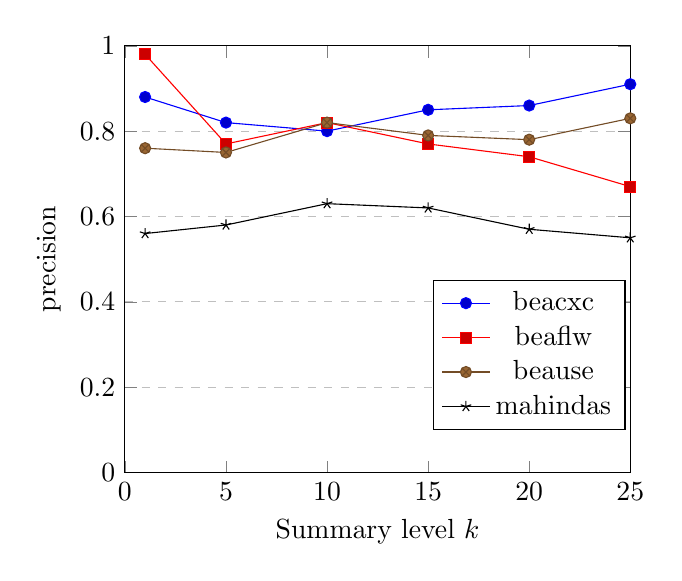
\begin{tikzpicture}
        \begin{axis}[
            xlabel={Summary level $k$},
            ylabel={precision},
            xmin=0, xmax=25,
            ymin=0, ymax=1.0,
            xtick={0,5,10,15,20,25},
            ymajorgrids=true,
            grid style=dashed,
            legend style={at={(0.8,0.1)},anchor=south},
            width=8cm,height=7cm]

            \addplot coordinates {
                (1,0.88)(5,0.82)(10,0.8)(15,0.85)(20,0.86)(25,0.91)
            };
            \addlegendentry{beacxc}
            
            \addplot coordinates {
                (1,0.98)(5,0.77)(10,0.82)(15,0.77)(20,0.74)(25,0.67)
            };
            \addlegendentry{beaflw}
        
            \addplot coordinates {
                (1,0.76)(5,0.75)(10,0.82)(15,0.79)(20,0.78)(25,0.83)
            };
            \addlegendentry{beause}
        
            \addplot coordinates {
                (1,0.56)(5,0.58)(10,0.63)(15,0.62)(20,0.57)(25,0.55)
            };
            \addlegendentry{mahindas}
        \end{axis}
    \end{tikzpicture}
    \caption{}
    %\caption{Precision of functional clusters generated by adapted FUSE algorithm}
    \label{fig:Precision}
\end{subfigure}

\begin{subfigure}[pt]{0.45\linewidth}
    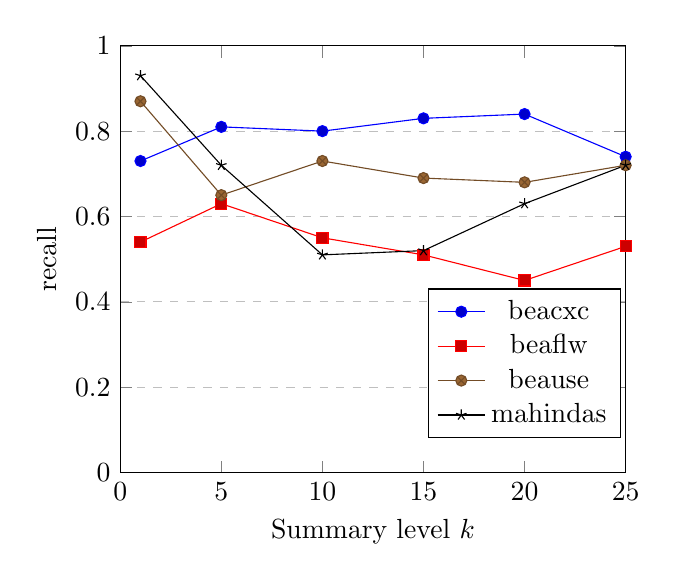
\begin{tikzpicture}
        \begin{axis}[
            xlabel={Summary level $k$},
            ylabel={recall},
            xmin=0, xmax=25,
            ymin=0, ymax=1.0,
            xtick={0,5,10,15,20,25},
            ymajorgrids=true,
            grid style=dashed,
            legend style={at={(0.8,0.08)},anchor=south},
            width=8cm,height=7cm]

            \addplot coordinates {
                (1,0.73)(5,0.81)(10,0.8)(15,0.83)(20,0.84)(25,0.74)
            };
            \addlegendentry{beacxc}
            
            \addplot coordinates {
                (1,0.54)(5,0.63)(10,0.55)(15,0.51)(20,0.45)(25,0.53)
            };
            \addlegendentry{beaflw}
        
            \addplot coordinates {
                (1,0.87)(5,0.65)(10,0.73)(15,0.69)(20,0.68)(25,0.72)
            };
            \addlegendentry{beause}
        
            \addplot coordinates {
                (1,0.93)(5,0.72)(10,0.51)(15,0.52)(20,0.63)(25,0.72)
            };
            \addlegendentry{mahindas}
        \end{axis}
    \end{tikzpicture}
    \caption{}
    %\caption{Recall of generated functional clusters from adapted FUSE algorithm}
    \label{fig:Recall}
\end{subfigure}
}


\caption{Cluster quality obtained using the adapted FUSE algorithm to summarize KGs from the financial sector. (a) Precision values. (b) Recall values}
\label{fig:ClustersQuality}
\end{figure*}


\begin{figure*}[!h]
\centering
\resizebox{2\columnwidth}{!}{
\begin{subfigure}[pt]{0.45\linewidth}
    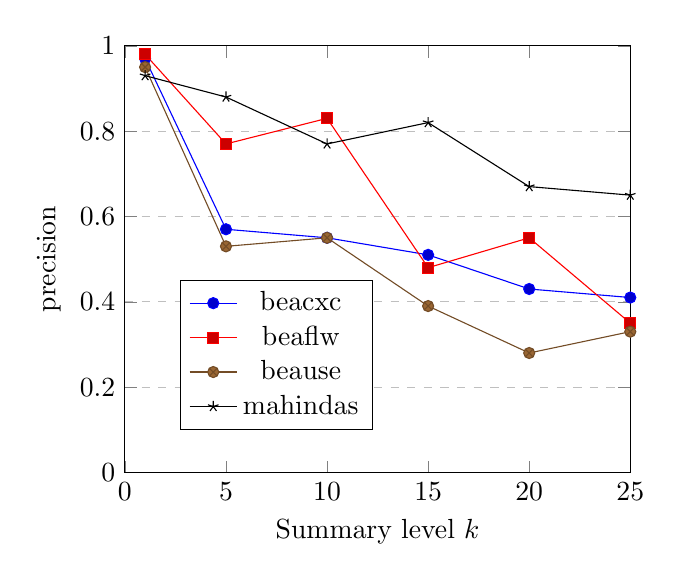
\begin{tikzpicture}
        \begin{axis}[
            xlabel={Summary level $k$},
            ylabel={precision},
            xmin=0, xmax=25,
            ymin=0, ymax=1.0,
            xtick={0,5,10,15,20,25},
            ymajorgrids=true,
            grid style=dashed,
            legend style={at={(0.3,0.1)},anchor=south},
            width=8cm,height=7cm]

            \addplot coordinates {
                (1,0.97)(5,0.57)(10,0.55)(15,0.51)(20,0.43)(25,0.41)
            };
            \addlegendentry{beacxc}
            
            \addplot coordinates {
                (1,0.98)(5,0.77)(10,0.83)(15,0.48)(20,0.55)(25,0.35)
            };
            \addlegendentry{beaflw}
        
            \addplot coordinates {
                (1,0.95)(5,0.53)(10,0.55)(15,0.39)(20,0.28)(25,0.33)
            };
            \addlegendentry{beause}
        
            \addplot coordinates {
                (1,0.93)(5,0.88)(10,0.77)(15,0.82)(20,0.67)(25,0.65)
            };
            \addlegendentry{mahindas}
        \end{axis}
    \end{tikzpicture}
    \caption{}
    %\caption{Precision of clusters generated the graph-based $k-means$ algorithm}
    \label{fig:Precision}
\end{subfigure}

\begin{subfigure}[pt]{0.45\linewidth}
    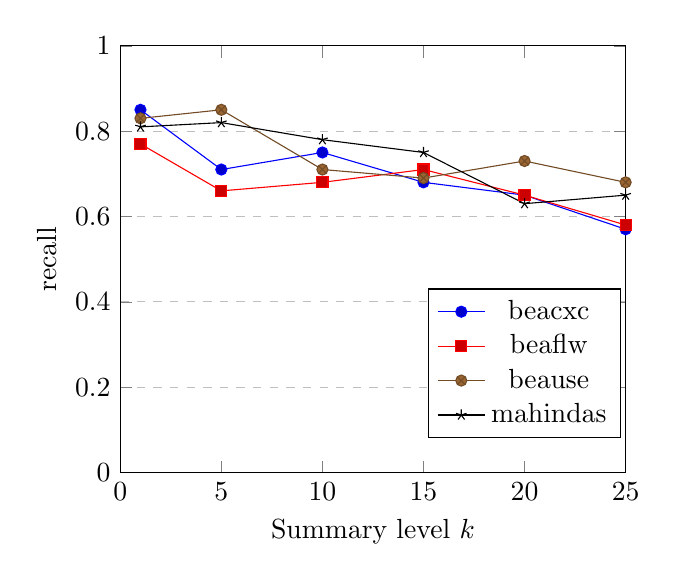
\begin{tikzpicture}
        \begin{axis}[
            xlabel={Summary level $k$},
            ylabel={recall},
            xmin=0, xmax=25,
            ymin=0, ymax=1.0,
            xtick={0,5,10,15,20,25},
            ymajorgrids=true,
            grid style=dashed,
            legend style={at={(0.8,0.08)},anchor=south},
            width=8cm,height=7cm]

            \addplot coordinates {
                (1,0.85)(5,0.71)(10,0.75)(15,0.68)(20,0.65)(25,0.57)
            };
            \addlegendentry{beacxc}
            
            \addplot coordinates {
                (1,0.77)(5,0.66)(10,0.68)(15,0.71)(20,0.65)(25,0.58)
            };
            \addlegendentry{beaflw}
        
            \addplot coordinates {
                (1,0.83)(5,0.85)(10,0.71)(15,0.69)(20,0.73)(25,0.68)
            };
            \addlegendentry{beause}
        
            \addplot coordinates {
                (1,0.81)(5,0.82)(10,0.78)(15,0.75)(20,0.63)(25,0.65)
            };
            \addlegendentry{mahindas}
        \end{axis}
    \end{tikzpicture}
    \caption{}
    %\caption{Recall of generated clusters generated by the graph-based $k-means$ algorithm}
    \label{fig:Recall}
\end{subfigure}
}


\caption{Cluster quality obtained using the graph-based $k-means$ algorithm to summarize KGs from the financial sector. (a) Precision values. (b) Recall values}
\label{fig:ClustersQualityClassical}
\end{figure*}

\textbf{Define a subset of visual data exploration tasks}
The following three tasks associated with the decision-making 
process in the financial sector are selected to conduct
the usability assessment:

\begin{enumerate}
    \item \textbf{FIBO01}: Observe the neighbors of the \textit{mean} term.
    \item \textbf{FIBO02}: Observe the relationships associated with the \textit{geopolitical entity} node. 
    \item \textbf{FIBO03}: Identify two types of relationships.
\end{enumerate}

\textbf{Select a group of analysts}. The tasks mentioned above were performed by
two analysts familiarized with graphs concepts and exploratory data analysis.

\textbf{Fix the layout algorithm}. The algorithm selected to generate the layout of the 
analyzed summary is the Fruchterman-Reingold algorithm.

\subsubsection{Analyze visual data exploration tasks}
\textbf{Measure time to complete every task}
As it is suggested in \cite{Camarillo20}, the efficiency of the obtained visual representation 
is measured by recording the analysis session where every user completes the visual exploration
tasks. After completing each task, the recording is stopped and the duration of this video represents
the value of the time needed to compute the efficiency metric. The efficiency of the visual 
representation is computed using the following formula:

\begin{equation}
  Efficiency = \frac{\sum_{j=1}^{R} \sum_{i=1}^{N} \frac{n_{ij}}{t_{ij}}}{NR}
  \label{eq:Efficiency}
\end{equation}

Where N is the number of tasks, R is the number of users, if the user
successfully completes the $i-th$ task $n_{ij} = 1$ otherwise  $n_{ij} = 0$
and $t_{ij}$ represents the time spent by $j-th$ user to complete the $i-th$
task. In Figure \ref{fig:Efficiency}, the visualized clustering result is 
16\% less efficiency for tasks \textbf{FIBO02} and \textbf{FIBO03}
compared with task \textbf{FIBO01}.

\begin{figure}[ht]
    \centering
    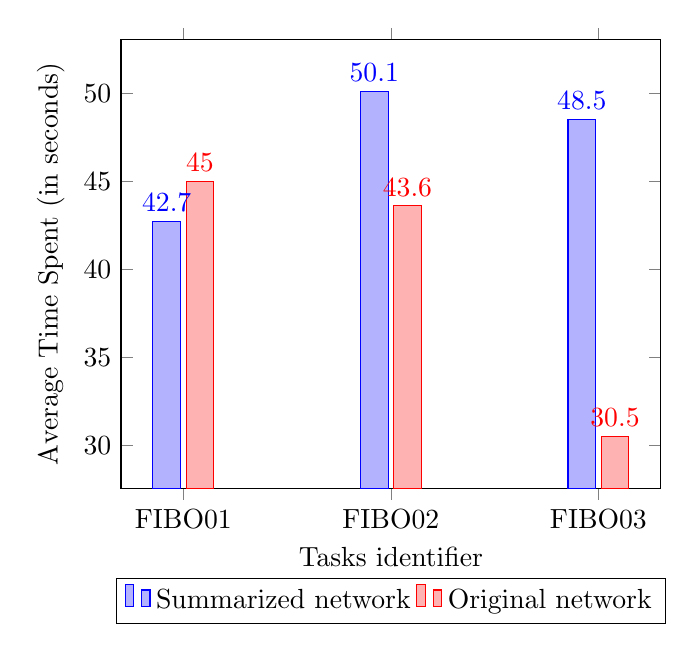
\begin{tikzpicture}
    \begin{axis}[
    ybar,
    enlargelimits=0.15,
    ylabel={Average Time Spent (in seconds)},
    xlabel={Tasks identifier},
    legend style={at={(0.5,-0.2)},
    anchor=north,legend columns=-1},
    %width=0.8*\textwidth,
    %height=9cm,
    %bar width=40pt,
    symbolic x coords={FIBO01,FIBO02,FIBO03},
    xtick=data,
    nodes near coords,
    nodes near coords align={vertical}
    ]
            \addplot
            coordinates {(FIBO01,42.7) (FIBO02,50.1) (FIBO03,48.5)};
            
            \addplot
            coordinates {(FIBO01,45.0) (FIBO02,43.6) (FIBO03,30.5)};
            
            \legend{Summarized network, Original network}
        \end{axis}
    \end{tikzpicture}
    \caption{Efficiency of visual data exploration tasks performed on functional summaries}
    \label{fig:Efficiency}
\end{figure}

\subsection{Discussion}

The modified FUSE algorithm suggests that the summary level 
do not affect precision values. For \textit{beacxc} and \textit{beause}
datasets, precision reaches 0.82 when summary level is $k = 25$. The
only network in which precision decreases when the summary level is increased
is \textit{beaflw}, falling out to 0.76 when $k = 25$. The lowest precision was
observed for the clusters computed for the \textit{mahindas} network, which barley 
exceeds 0.6 for $k = 10$ and $k = 15$. Precision values of the modified FUSE algorithm
are better than the precision values obtained
with the $k-means$ algorithm. With $k = 25$, the maximum precision value for $k-means$
clustering is 0.65, which is the barley greater than the minimum precision value obtained
by the adapted FUSE algorithm.

On the other hand, recall values show a poor quality for clusters computed when the
level of summary is increased compared with the $k-means$ clustering strategy. For \textit{beaflw} 
network, the recall value is 0.54 when the summary level is $k = 1$, when the summary level $k$
increases to $25$, this metric falls out to 0.53. In general, this pattern of
decreasing the recall value while the summary level increases occurs for 
the four summarized networks. In contrast, the recall values observed in
experiments with the $k-means$ clustering show a stability trend when the summary level increases. When
the summary level is 25, the minimum recall value is 0.57 ($beacxc$ network).

Regarding visual representation efficiency of the \textit{mahindas} network, the
user interface needs to be improved. The analysts that fulfill the visual 
exploration tasks using the summarized network invested more time than the 
time spent to perform the analysis tasks by visualizing the entire graph. For
a common task, such as \textbf{FIBO02}, users spent 50.1 seconds in average.
Future work is on improving the usability evaluation of the 
visualization systems that manage summarized networks due to the poor performance of the user interface.

\section{Conclusion}

In this paper an adaptation of the FUSE algorithm is utilized to summarize knowledge graphs. In order to generate the functional clusters, the structural knowledge information value is introduced as a parameter to determine whether a node from the original graph belongs or not to the initial clusters. Public data from the financial sector is used to validate the initial hypothesis of the applicability of the FUSE algorithm to generate functional clusters for different biology domains.  Then,  summarized networks are visualized and the efficiency of this visual representation is measured to evaluate the usability of functional clusters for exploratory data analysis tasks.
\end{comment}

\bibliography{vis} 
\bibliographystyle{IEEEtran}
\EOD

\end{document}
